\def\thesispath{/home/lukas/Desktop/project/independence/project/thesis}
% HEADER -----------------------------------------------------------------------
\documentclass[10pt, mathserif]{beamer}


\usepackage{hyperref}
\hypersetup{
    colorlinks=true,
    linkcolor=primary_0,
    citecolor=neutral_1,
    urlcolor=red,
    pdfauthor={Lukas Scheucher},
    pdfcreator={Lukas Scheucher},   % creator of the document
    pdfproducer={Lukas Scheucher}, % producer of the document
    linktoc=all
}

\usetheme{CambridgeUS}
\setbeamertemplate{navigation symbols}{}
\useoutertheme[subsection=false]{miniframes}

\setbeamercolor{block body}{bg=yellow!23}
\setbeamercolor{block title}{bg=purple!100!black!140, fg=white}
\setbeamercolor{footline}{fg=gray!100}
\setbeamercolor{item}{fg=purple!100!black!150,bg=purple!100!black!150}
\setbeamercolor*{title}{fg=purple!100!black!150,bg=lightgray!50}
\setbeamercolor*{author}{fg=blue}
\setbeamercolor*{author in head/foot}{fg=blue,bg=gray!15}
\setbeamercolor*{author in head/foot}{fg=black,bg=gray!15}
\setbeamercolor*{date in head/foot}{fg=black,bg=gray!25}
\setbeamercolor*{frametitle}{fg=purple!100!black!150, bg=gray!15}
\setbeamerfont{footl}{size=\tiny}
\usefonttheme[onlylarge]{structuresmallcapsserif}
\setbeamerfont{frametitle}{size=\normalsize}

\setbeamertemplate{footline}
{
  \leavevmode%
  \hbox{%
  \begin{beamercolorbox}[wd=.4\paperwidth,ht=1.6ex,dp=1ex,center]{author in head/foot}%
    \usebeamerfont*{footl}\insertshortauthor~~(\insertshortinstitute)
  \end{beamercolorbox}%
  \begin{beamercolorbox}[wd=.6\paperwidth,ht=1.6ex,dp=1ex,right]{date in head/foot}%
    \usebeamerfont*{footl}\insertshortdate{}\hspace*{2em}
    \insertframenumber{} / \inserttotalframenumber\hspace*{2ex}
  \end{beamercolorbox}}
  \vskip0pt%
}



\usepackage{amsmath, amstext, amssymb, latexsym, psfrag, soul, cancel, relsize}
\usepackage{graphicx, color, colortbl, epsfig, subfigure, booktabs, animate}
\usepackage{tikz}
\usetikzlibrary{shapes,arrows}
\usepackage[percent]{overpic}


\usetikzlibrary{positioning}
\usetikzlibrary{calc}
\usepackage{pgfplots}
\usepackage{pgfplotstable}
\usepgfplotslibrary{groupplots}

% Define block styles
\tikzstyle{decision} = [diamond, draw, fill=yellow!80, 
                        text width=4.5em, text badly centered, node distance=2cm, inner sep=0pt]
\tikzstyle{block}  = [rectangle, draw, fill=black!20, 
                     text width=8em, text centered, rounded corners, minimum height=1em]
\tikzstyle{block1} = [rectangle, draw, fill=blue!30, 
                     text width=8em, text centered, rounded corners, minimum height=1em]
\tikzstyle{block3} = [rectangle, draw, fill=red!50, 
                     text width=8em, text centered, rounded corners, minimum height=1em]
\tikzstyle{block2} = [rectangle, draw, fill=green!40, 
                     text width=8em, text centered, rounded corners, minimum height=1em]
\tikzstyle{block4} = [rectangle, draw, fill=yellow!80, 
                     text width=8em, text centered, rounded corners, minimum height=1em]
\tikzstyle{blocke} = [rectangle, draw, fill=yellow!25, 
                     text width=16em, text centered, rounded corners, minimum height=2em]
\tikzstyle{line} = [draw, -latex']

\tikzstyle{blocka}  = [rectangle, draw, fill=neutral_4, 
                     text width=4em, text centered, rounded corners, minimum height=1em]
                     
\tikzstyle{blockb}  = [rectangle, draw, fill=neutral_0, 
                     text width=4em, text centered, rounded corners, minimum height=1em]


%%%%%%%%%%%%%%%%%%%%%%%%%%%%%%%%%%
\newcommand{\Rbb}{\ensuremath{\mathbb{R} }}
\newcommand\mubold{{\ensuremath{\boldsymbol{\mu}}}}
\newcommand{\Jcal}{\ensuremath{\mathcal{J}}}
\newcommand{\func}[3]{\ensuremath{#1 : #2 \rightarrow #3}}
\newcommand{\Dcal}{\ensuremath{\mathcal{D}}}
\newcommand{\Fcal}{\ensuremath{\mathcal{J}}}

\newcommand\cbold{\ensuremath{\mathbf{c}}}
\newcommand{\pder}[2]{\ensuremath{\dfrac{\partial #1}{\partial #2}}} %1st partial derivative
\newcommand{\oder}[2]{\ensuremath{\dfrac{\mathrm{d} #1}{\mathrm{d} #2}}} %1st ordinary derivative

\newcommand\Rbold{\ensuremath{\mathbf{R}}}
\newcommand\ubold{\ensuremath{\mathbf{u}}}
\newcommand\wbold{\ensuremath{\mathbf{w}}}
\newcommand\Fbold{\ensuremath{\mathbf{F}}}
\newcommand\fbold{\ensuremath{\mathbf{f}}}
\newcommand\xbold{\ensuremath{\mathbf{x}}}
\newcommand\nbold{\ensuremath{\mathbf{n}}}
\newcommand\C{\mathcal{C}}
\newcommand\dC{\partial\mathcal{C}}
\newcommand\n{\boldsymbol{n}}
\newcommand\K{\mathcal{K}}

\newcommand{\Et}{E^t}
\newcommand{\IdxM} {\mathbb{I}}
\newcommand{\vel}{\boldsymbol{v}}
\newcommand{\mm}{\boldsymbol{m}}
\newcommand{\dsddt}[1] {\dfrac{\partial{#1}}{\partial{t}}}
\newcommand{\Div}[1] { \boldsymbol{\nabla} \!\dotprod #1 }
\newcommand{\vzero}{\boldsymbol{0}}
\newcommand{\wall}{\mathrm{wall}}
%%%%%%%%%%%%%%%%%%%%%%%%%%%%%%%%%%

\title[]{\large{Analytical and Numerical Approaches for the Computation of Aeroelastic Sensitivities Using the Direct and Adjoint Methods}}
\author[Scheucher]{Lukas Scheucher}
\institute[Stanford]{Stanford University}
\date[SMaster thesis]{October 2016 - June 2017}
\newcommand{\backupbegin}{
   \newcounter{finalframe}
   \setcounter{finalframe}{\value{framenumber}}
}
\newcommand{\backupend}{
   \setcounter{framenumber}{\value{finalframe}}
}


\usepackage{hhline}


\usepackage{color}
\usepackage{xcolor}
\usepackage{soul}
\definecolor{hlcolorblue}{RGB}{126,215,255}
\definecolor{hlcolorgreen}{RGB}{126,255,175}
\definecolor{hlcolororange}{RGB}{246,194,115}
\definecolor{hlcoloryellow}{RGB}{255,243,113}
\definecolor{hlcolorpurple}{RGB}{215,163,232}
\DeclareRobustCommand{\hltblue}[1]{{\sethlcolor{hlcolorblue}\hl{#1}}}
\DeclareRobustCommand{\hltgreen}[1]{{\sethlcolor{hlcolorgreen}\hl{#1}}}
\DeclareRobustCommand{\hltorange}[1]{{\sethlcolor{hlcolororange}\hl{#1}}}
\DeclareRobustCommand{\hltyellow}[1]{{\sethlcolor{hlcoloryellow}\hl{#1}}}
\DeclareRobustCommand{\hltpurple}[1]{{\sethlcolor{hlcolorpurple}\hl{#1}}}
\newcommand{\hleblue}[1]{\colorbox{hlcolorblue}{$\displaystyle{#1}$}}
\newcommand{\hlegreen}[1]{\colorbox{hlcolorgreen}{$\displaystyle{#1}$}}
\newcommand{\hleorange}[1]{\colorbox{hlcolororange}{$\displaystyle{#1}$}}
\newcommand{\hleyellow}[1]{\colorbox{hlcoloryellow}{$\displaystyle{#1}$}}
\newcommand{\hlepurple}[1]{\colorbox{hlcolorpurple}{$\displaystyle{#1}$}}


\def\maathunderline#1#2{\color{#1}\underline{{\color{black}#2}}\color{black}}

\newsavebox\MBox
\newcommand\mathunderline[2][red]{{\sbox\MBox{$#2$}%
  \rlap{\usebox\MBox}\color{#1}\rule[-1.2\dp\MBox]{\wd\MBox}{2.0pt}}}

\DeclareRobustCommand{\hlt}[2]{{\sethlcolor{#1}\hl{#2}}}
\newcommand{\hle}[2]{\colorbox{#1}{$\displaystyle{#2}$}}




% beamer color sheme

%\setbeamercolor*{palette primary}{bg=yellow, fg = green}
%\setbeamercolor*{palette secondary}{bg=orange, fg = black}
\setbeamercolor*{palette tertiary}{bg=primary_0, fg = white}%title bar
%\setbeamercolor*{palette quaternary}{bg=purple, fg = black}


%colors for text highlighting
\definecolor{hlcolor_blue}{RGB}{126,215,255}
\definecolor{hlcolor_green}{RGB}{126,255,175}
\definecolor{hlcolor_orange}{RGB}{246,194,115}
\definecolor{hlcolor_yellow}{RGB}{255,243,113}
\definecolor{hlcolor_purple}{RGB}{215,163,232}

%tikz color list
\definecolor{list1_1}{RGB}{0,101,189}
\definecolor{list1_2}{RGB}{156,157,159}
\definecolor{list1_3}{RGB}{162,173,0}
\definecolor{list1_4}{RGB}{227,114,34} 
\definecolor{list1_5}{RGB}{152,198,234}


%\definecolor{list1_1}{RGB}{246,81,29}
%\definecolor{list1_2}{RGB}{255,180,0}
%\definecolor{list1_3}{RGB}{0,166,237}
%\definecolor{list1_4}{RGB}{127,184,0}
%\definecolor{list1_5}{RGB}{13,44,84}


\pgfplotscreateplotcyclelist{markerlist}{
list1_1, thick, solid, mark=*\\%
list1_2, thick, solid, mark=asterisk\\%
list1_3, thick, solid, mark=diamond*\\%
list1_4, thick, solid, mark=triangle\\%
list1_5, thick, solid, mark=square\\%
}

\pgfplotscreateplotcyclelist{linelist}{
list1_1, solid\\%
list1_2, solid\\%
list1_3, solid\\%
list1_4, solid\\%
list1_5, solid\\%
}

\definecolor{lightgrey}{RGB}{200,200,200}
\definecolor{nassitextcolor}{RGB}{0,0,200}
\newcommand{\abbrevation}[2]{\newcommand{#1}{#2}}
\abbrevation{\SQP}{SQP}      %Sequential Quatdratic Programming

%%==============================%
% OPERATORS
% Representation of scalars, tensors and other quantities
%==============================%
\newcommand{\s}[1]{#1}                        %Scalar quantity with{a}
\renewcommand{\v}[1]{\mathcal{\boldsymbol{#1}}}      %Vector quantity with{a}
\newcommand{\m}[1]{\mathcal{\boldsymbol{#1}}}      %Matrix quantity with{A}
\renewcommand{\c}[1]{\mathnormal{#1}}              %continous quantity with{A,a}
\renewcommand{\d}[1]{\mathrm{#1}}                  %discrete quantity  with{A,a}
\renewcommand{\it}[1]{{#1}^{(k)}}                  %Iteration index in the optimization loop            with{a}
\newcommand{\ito}[1]{{#1}^{(k)}}                   %Iteration index in the optimization loop            with{a}
\newcommand{\its}[1]{{#1}^{(n)}}                   %Iteration index in thestaggered algorithm           with{a}
\newcommand{\fic}[1]{\bar{#1}}                     %Fictious entity                                     with{A}
\newcommand{\order}[1]{\mathcal{O}(#1)}            %Order of magnitude                                  with{A}


\newcommand{\itn}[1]{{#1}^{(0)}}                   %Iteration index 0                                   with{A}
\newcommand{\itss}[1]{{#1}^{(n+1)}}                %Iteration index in thestaggered algorithm           with{A}
\newcommand{\pd}{\mathrm{\partial}}                %TODO check whether I need the partial or not        with{A}
\renewcommand{\vec}[1]{\boldsymbol{#1}}            %Vector                                                                       with{A}
\newcommand{\abs}[1]{\lvert#1\rvert}               %Norm of a vector                                                             with{A}
\newcommand{\expression}[1]{\textit{#1}}           %To mark a new term beein introduced
\newcommand{\prim}[1]{\tilde{#1}}                  %To mark a variabla as being expressen in primitive variables
\newcommand{\dvec}[1]{\boldsymbol{ \mathsf{#1} } } %discrete vector represenation of a scalar field     with{A}
\newcommand{\dmat}[1]{\boldsymbol{\mathsf{#1}}}    %discrete vector represenation of a tensor field     with{A}


%%==============================%
% OPERATORS
% Algebraic operations
%==============================%
\newcommand{\T}[1]{{#1}^{T}}                      %Transpose of a tensor                with{A}
\newcommand{\inv}[1]{ {#1}^{-1}}                  %Inverse of a tensor                  with{A}
\newcommand{\av}[1]{\bar{#1}}                     %Average component of a quantity      with{a}
\newcommand{\fluc}[1]{{#1}'}                      %Fluctuating component of a qunatity  with{a}
\newcommand{\norm}[1]{\left\lVert#1\right\rVert}  %Norm of a quatntity                  with{a}


%%==============================%
% OPERATORS
% Analytic operations
%==============================%
\newcommand{\dderivtime}[1]{\ddot{#1}}                        %Second time derivative at a fixed refrence position                   with{A}
\newcommand{\derivtime}[1]{\dot{#1}}                          %First time derivative at a fixed reference position                   with{A}
\newcommand{\pdfrac}[2]{\frac{\pd #1}{\pd #2}}                %partial derivative of one argument with respect to the other          with{A&B}
\newcommand{\ppdfrac}[2]{\frac{\pd^{2} #1}{\pd {#2}^{2}}}     %Second partial derivative of one argument with respect to the other   with{A&B}
\newcommand{\mfrac}[2]{\frac{D #1}{D #2}}                     %Material time derivative                                              with{A&B}
\renewcommand{\tfrac}[2]{\frac{\mathrm{d} #1}{\mathrm{d} #2}} %First total derivative of one argument with respect to the other      with{A&B}




\renewcommand{\st}[1]{{#1}^{0}}                  %Value at steady state
\newcommand{\0}{\textcolor{lightgrey}{0}}
\newcommand{\tensor}[1]{\mathcal{\boldsymbol{#1}}} %Vector quantity with{a}
\newcommand{\scalar}[1]{\s #1}                        %Scalar quantity with{a}


%==============================
% SYMBOLS
% 3-field formulations
%==============================
\newcommand{\EOSstruct}{\mathcal{S}}     %State equation of the structure
\newcommand{\EOSmesh}  {\mathcal{D}}     %State equation of the mesh
\newcommand{\EOSfluid} {\mathcal{F}}     %State equation of the fluid
\newcommand{\mms}       {\vec{x}}        %Fluid mesh motion
\newcommand{\mmsad}       {\vec{a}_{\vec{x}}}        %Adjoint fluid mesh motion
\newcommand{\fstate}    {\vec{w}}        %Fluid state vector
\newcommand{\fstatead}{\vec{a}_{\vec{w}}}  %Adjoint fluid state vector
\newcommand{\fstateprim}{\prim{\fstate}}        %Primitive ffluid state vector
\newcommand{\dfstate}    {\dvec{w}}        %Discrete fsluid state vector
\newcommand{\structdisp}{\vec{u}}        %Structure displacement
\newcommand{\structdispad}{\vec{a}_{\vec{u}}}        %Adjoint structure displacement
\newcommand{\load}{\vec{P} }          %Fluid load TODO
\newcommand{\fload}{\vec{P}_F}           %Fluid load
\newcommand{\sload}{\vec{P}_T}           %Structure load
\newcommand{\jactwo}{\tensor{H}_2}       %Second order Jacobian
\newcommand{\ifaceprojFtoS}{\dmat{T}_p}  %Interface projection matrix from fluid to structure mesh
\newcommand{\ifaceprojStoF}{\dmat{T}_u}  %Interface projection matrix from structure to fluid mesh
\newcommand{\fstaterans}{\fstate_{RANS}}   %Augumentes fluid state vector in the \ac{RANS} formulation
\newcommand{\turbulenceparam}{\chi}        %Additional fluid state variable introduced by the turbulence model
\newcommand{\turbparamvec}{\dvec{\chi}}        %Additional fluid state variable introduced by the turbulence model
\newcommand{\turbulencesource}{\mathsf{S}} %Source term in the \ac{RANS} equations
\newcommand{\fluxmatconv}{\dmat{F}}       %Convective part of the flux matrix
\newcommand{\fluxmatdiff}{\dmat{G}}       %diffusive part of the flux matrix
\newcommand{\turbmat}{\dmat{S}}           %Turbulence term
\newcommand{\cellvolmat}{\dmat{A}}        %Diagonal matrix with vell volumes

\newcommand{\specificwork}{\vec{w}}       %specific work



%==============================%
% SYMBOLS
% Optimization
%==============================%
\newcommand{\costfunc}{z}               %Target cost function
\newcommand{\eqctr}{\vec{h}}            %Equality constraints
\newcommand{\numeqctr}{n_{\vec{h}}}     %Number of equality constraints
\newcommand{\neqctr}{\vec{g}}           %Non-equality constraints
\newcommand{\numneqctr}{n_{\vec{g}}}    %Number of non-equality constraints
\newcommand{\absvar}{s}                 %Abstract optimazation variable
\newcommand{\absvars}{\vec{s}}          %Vector of abstract optimization variables
\newcommand{\optcrit}{q}                %Optimization criterium
\newcommand{\optcrits}{\vec{\optcrit}}  %Vector of optimization criteria
\newcommand{\physvars}{\vec{d}}         %Physical design parameters
\newcommand{\Lagfunc}{L}                %Lagrangian function of the optimization problem
\newcommand{\lagmultseq}{\vec{\eta}}    %Lagrange multipliers of the equality constraints
\newcommand{\lagmultsneq}{\vec{\gamma}} %Lagrange multipliers of the inequality constraints
\newcommand{\adjoints}{\vec{a}}         %Adjoint solutions
\newcommand{\tolsa}{\epsilon^{SA}}      %Specified tolerance in the Sensitivity analysis


%==============================%
% SYMBOLS
% Fluid Mechanics
%==============================%
\newcommand{\fluxesconv}{\mathcal{F}} %Convective fluxes
\newcommand{\fluxesdiff}{\mathcal{G}} %Diffusive fluxes
\newcommand{\dens}{\rho}              %Density
\newcommand{\pres}{p}                 %Pressure
\newcommand{\fluidvel}{\vec{v}}       %Fluid velocity vector
\newcommand{\fluidvelcomp}{v}         %Fluid velocity vector
\newcommand{\fluidvelx}{{v_1}}          %Fluid velocity in x-direction
\newcommand{\fluidvely}{{v_2}}          %Fluid velocity in y-direction
\newcommand{\fluidvelz}{{v_3}}          %Fluid velocity in z-direction
\newcommand{\energytot}{E}            %Total energies
\newcommand{\energyint}{e}            %Internal energy
\newcommand{\eye}{\dmat{I}}           %Identity matrix
\newcommand{\fluidstrain}{\tensor{\epsilon}}    %Deviatoric fluid stress tensor
\newcommand{\fluidstress}{\tensor{\tau}}    %Deviatoric fluid stress tensor
\newcommand{\fluidstresscomp}{\tau}   %Deviatoric fluid stress tensor
\newcommand{\thermcond}{k}            %Thermal conductivity of the fluid
\newcommand{\temp}{T}                 %Fluid temperature
\newcommand{\heatfluxcomp}{q}         %Heat flux comopnenent
\newcommand{\heatflux}{\vec{\heatfluxcomp}} %Heat flux vector
\newcommand{\viscosdyn}{\mu}          %Dynamic viscosity
\newcommand{\viscoskin}{\nu}          %Kinematic viscosity
\newcommand{\reynolds}{RE}            %Reynolds number
\newcommand{\specheatratio}{\gamma}   %Specific heat ratio
\newcommand{\jac}{\mathcal{H}}        %Jacoian matrix
\newcommand{\fluxjac}{\mathcal{A}}    %Flux Jacobian
\newcommand{\jaceigvecs}{\tensor{P}}  %Matrix that contains the eigenvectors of the jacobian matrix of $\fluxmatconv$
\newcommand{\jaceigvals}{\tensor{\Lambda}}  %Diagonal matrix that contains the eigenvalues of the jacobian matrix of $\fluxmatconv$
\newcommand{\roeavgfunc}{\tensor{M}}  %Averaging function associated with the Roe flux


\newcommand{\normal}{\vec{n}}        %Symbol for dyadic product
\newcommand{\normalx}{n_1}        %Symbol for dyadic product
\newcommand{\normaly}{n_2}        %Symbol for dyadic product
\newcommand{\normalz}{n_3}        %Symbol for dyadic product
\newcommand{\testfunc}{\phi}         %Variational test function
\newcommand{\vertex}{\boldsymbol{X}}  %Mesh vertex
\newcommand{\vertexset}{\mathsf{\kappa}} %Set of vertices
\newcommand{\fluxesnum}{\boldsymbol{\phi}} %numerical flux
\newcommand{\roeavgmat}{\tensor{A}_{\text{Roe}}}  %Averaging matrix of the Roe flux
\newcommand{\eigval}{\lambda}         %Eigen value
\newcommand{\sspeed}{c} %Speed of sound

\newcommand{\dyadic}{\otimes}        %Symbol for dyadic product
\newcommand{\REF}{\textbf{REF}}
%%%==============================%
%%% SYMBOLS
%%% Fluid Analysis
%%%==============================%
%%\newcommand{\sate}{w}
%%\newcommand{•}{•}
%%\newcommand{•}{•}
%%\newcommand{•}{•}
%%\newcommand{\statevec}{\vec{\state}}


%==============================%
% SYMBOLS
% Sturctural Analysis
%==============================%
\newcommand{\stiffmat}{\dmat{K}}               %\ac{FE} stiffness matrix
\newcommand{\disp}{u}                          %Displacement vector
\newcommand{\dispvec}{\dvec{\disp}}            %Discrete displacement vector
\newcommand{\motion}{\vec{x}}                  %Mesh motion
\newcommand{\ifacedisp}{d}                     %Interface displacement
\newcommand{\ifacedispvec}{\dvec{\ifacedisp}}  %Interface displacement 


%==========================================
% SYMBOLS
% Fluid Structure Interaction
%==========================================
\newcommand{\strucstateq}{\mathcal{P}}         %State equation of the structure
\newcommand{\fluidstateq}{\mathcal{F}}         %State equation of the fluid
\newcommand{\mmsstateeq}{\mathcal{D}}          %State equation of the mesh motion


%=============================================================================%
% Nassi-Schneidermann auxiliary commands                                      %
%=============================================================================%

%commands for the text part of the dioagrams
%the bold command is typcally used for TODO
%there is now automatic line wrapping in strtuktex, so the  second command is
% used if the text becomes too long
\newcommand{\nassitext}[2]{\makebox[#1\textwidth]{\textit{\textcolor{nassitextcolor}{\small #2}}\hfill}}
\newcommand{\nassitextbold}[2]{\makebox[#1\textwidth]{\textbf{\textit{\textcolor{nassitextcolor}{\small #2}}}\hfill}}
\newcommand{\nassitexttwolines}[3]{\nassitext{#1}{#2}\hspace*{\hsize}\linebreak \nassitext{\df2}{#3}}

\newcommand{\tablesix}[6]{
\begin{tabular}{|c|l|l|}
\hline
  \parbox[t]{2mm}{\multirow{3}{*}{\rotatebox[origin=c]{90}{Eulerian}}}  & EULER & #1 \\
  \hhline{~--}                                                          & NSG   & #2 \\
  \hhline{~--}                                                          & RANS  & #3 \\
\hline
  \parbox[t]{2mm}{\multirow{3}{*}{\rotatebox[origin=c]{90}{ALE}}}       & EULER & #4 \\
  \hhline{~--}                                                          & NSG   & #5 \\
  \hhline{~--}                                                          & RANS  & #6 \\
\hline
\end{tabular}
}

% ------------------------------------------------------------------------------

\usepackage[backend=biber,style=authortitle]{biblatex}
%\begin{filecontents}{myreferences.bib}
%\input{/home/lukas/Desktop/project/independence/project/thesis/bibliography.bib}
%\end{filecontents}

\addbibresource{\thesispath/bibliography.bib}

\AtBeginSection[]
{
  \begin{frame}<beamer>
    \frametitle{Outline for section \thesection}
    \tableofcontents[currentsection]
  \end{frame}
}

\begin{document}

%\input{/home/lukas/Desktop/project/independence/project/thesis/bibliography.bib}

% TITLE FRAME ------------------------------------------------------------------
\begin{frame}
   \titlepage
   \begin{figure}[!ht]
   \centering
    
\includegraphics[width=0.35\linewidth]{Fig/logo_stanford}
   \end{figure}
\end{frame}

\begin{frame}{Overview}
\tableofcontents
\end{frame}
% -----------------------------------------------------------------------------



% MAIN PART -------------------------------------------------------------------
\section{Introduction}


%-----------------------------------------------------------------------------------------------------

\begin{frame}
  \frametitle{Motivation}
  \only<1>{\framesubtitle{ Basics}}
  \only<2>{\framesubtitle{$\rightarrow$ Why Sensitivity Analysis?}}
  \only<3>{\framesubtitle{$\rightarrow$ Why Embedded framework?}}
  \only<4->{\framesubtitle{$\rightarrow$ Why analytic approach?}}
  \begin{itemize}
    \item Aerodynamic optimization
     \begin{itemize}
       \item \textbf<2>{Gradient based}
       \item \textbf<2>{Take the human out of the loop}
     \end{itemize}
    \item Requirements on CFD
      \begin{itemize}
      \item \textbf<3>{Complex flows (transonic, turbulent \dots) and high Reynolds numbers}
      \item Well-resolved boundary layers and flow features
      \item Steady/unsteady flows
      \item \textbf<4>{Numerical accuracy, solver robustness and short turn-around time}
      \item \textbf<3>{Moderate to highly complex geometries}
      \end{itemize}
    \item Requirements on design and optimization 
      \begin{itemize}
      \item Automatic framework
      \item Efficient optimization algorithms
      \item \textbf<3>{Large number of design variables}
      \item Multi-point design and multi-disciplinary design optimization
      \item Geometrical/engineering constraints 
      \end{itemize}
   \end{itemize}
   \onslide<3>{$\rightarrow$\textbf{Embedded framework}}\\
   \onslide<4>{$\rightarrow$\textbf{Analytic Sensitivities}}
\end{frame}

\note[itemize]
{
\item{First note.}
\item{Second note.}
\subitem{Test}
}


%-----------------------------------------------------------------------------------------------------

\begin{frame}
  \frametitle{The AERO-Suite\footcite{Aerof}~\footcite{Aeros}}
  \framesubtitle{Workflow}
%  \centering
  \def\vert{0.5cm}
  \def\horz{0.5cm}
  \centering
      \scalebox{0.8}{\begin{tikzpicture}[scale=1.0]
        \node [block3]                                      (aerof) {\textbf<2>{Aero-F}};
        \node [block3, below right=\vert and \horz of aerof]   (matcher) {Matcher};
        \node [block3, above right=\vert and \horz of matcher] (aeros) {Aero-S};
        \node [block3, below=\vert of matcher]             (sower) {Sower};
        \node [block3, below=\vert of sower]             (mesh) {Mesh};
        \node [block3, above right=\vert and \horz of aerof] (sowerr) {Sower};
        \node [block3, above=\vert of sowerr]             (xpexo) {xpexo};
        
        \node [block,below=\vert of mesh]             (gmsh) {GMSH};
        \node [block,above=\vert of xpexo]             (paraview) {Paraview};
        
        \draw[<->,dashed,thick] (aerof) -- (matcher);
        \draw[<->,dashed,thick] (aeros) -- (matcher);
        \draw[->,dashed,thick] (sower) -- (matcher);
        \draw[->,thick] (sower) -| (aerof);
        \draw[->,thick] (sower) -| (aeros);
        
        \draw[->,thick] (mesh) -- (sower);
        \draw[->,thick] (gmsh) -- (mesh);
        \draw[->,thick] (sowerr) -- (xpexo);
        \draw[->,thick] (xpexo) -- (paraview);
        
        \draw[->,thick] (aerof) |- (sowerr);
        \draw[->,thick] (aeros) |- (sowerr);
        
        \draw[darkgrey,thick,dashed] ($(gmsh.north west)+(-4.0,0.15)$)  rectangle ($(xpexo.north east)+(4.0,0.15)$);    %SDesign
     \end{tikzpicture}}
\end{frame}

%------------------------------------------------------------------------------

%\begin{frame}
%  \frametitle{Aerodynamic shape optimization}
%  \only<1>{\framesubtitle{-> Overview}}
%  \only<2>{\framesubtitle{-> Thesis focus}}
%  
%  \begin{columns}
%    \begin{column}{0.55\textwidth}
%      \scalebox{0.9}{\begin{tikzpicture}[scale=1.0,node distance = 1.2cm]
%        \node [block]                                      (init) {Initial geometry};
%        \node [block1, below of=init]                      (parameter) {Parameter change};
%        \node [block1, below= 1cm of parameter]                 (modify) {\textbf<2>{Shape}  \mbox{\textbf<2>{modification}}};
%        \node [block2, below= 1cm of modify]                    (mesh) {Mesh procedure};
%        \node [block3, below of=mesh]                      (simulation) {Flow simulation};
%        \node [decision, right of=parameter, node distance=3.5cm] (decide) {Optimum?};
%        \node [block4, right of=mesh, node distance=3.5cm] (optimize) {Gradient based optimization};
%        \node [block3, below of=simulation]                (objective) {\textbf<2>{Gradient of objective function \& constraints}}; 
%        \path [line] (init) -- (parameter);
%        \path [line] (parameter) -- (modify);
%        \path [line] (decide) -- (parameter);        
%        \path [line] (modify) -- (mesh);
%        \path [line] (mesh) -- (simulation);
%        \path [line] (simulation) -- (objective);   
%        \path [line] (objective) -| (optimize);
%        \path [line] (optimize) -- (decide);  
%        
%        \draw[darkgrey,thick,dotted] ($(parameter.north west)+(-0.2,0.15)$)  rectangle ($(parameter.south east)+(0.2,-0.45)$);    %SDesign
%        \draw[darkgrey,thick,dotted] ($(modify.north west)+(-0.2,0.15)$)  rectangle ($(modify.south east)+(0.2,-0.45)$);    %SDesign
%        \draw[darkgrey,thick,dotted] ($(mesh.north west)+(-0.2,0.15)$)    rectangle ($(objective.south east)+(0.2,-0.45)$); %Aero-F   
%        \draw[darkgrey,thick,dotted] ($(decide.north west)+(-1.2,0.6)$)   rectangle ($(optimize.south east)+(0.2,-0.45)$);  %Python
%        
%        \node [darkgrey,anchor=north east] at  ($(parameter.south east)+(0.0,0.0)$)                (aaa) {\texttt{Bash}};
%        \node [darkgrey,anchor=north east] at  ($(optimize.south east)+(0.0,0.0)$)                (aaa) {\texttt{Python}};
%%        \onslide<1>{\node [darkgrey,anchor=north east] at  ($(optimize.south east)+(0.0,0.0)$)                (aaa) {\texttt{Python}};};
%%        \onslide<2>{\node [black,anchor=north east] at  ($(optimize.south east)+(0.0,0.0)$)                (aaa) {\texbf{Python}};};
%        \node [darkgrey,anchor=north east] at  ($(objective.south east)+(0.0,0.0)$)                (aaa) {\texttt{Aero-F}};
%        \node [darkgrey,anchor=north east] at  ($(modify.south east)+(0.0,0.0)$)                (aaa) {\texttt{SDesign}};
%      \end{tikzpicture}}
%    \end{column}
%    \begin{column}{0.45\textwidth}
%      \begin{block}{Gradient based optimization}
%       \begin{itemize}
%       \item Requires objective function and constraints
%       \item Gradient of objective function and constraints
%       \end{itemize}
%       \end{block}
%      \begin{block}{How to compute the gradient}
%       \begin{itemize}
%       \item Finite difference
%       \item \textbf<2>{Direct approach}
%       \item Adjoint approach
%       \end{itemize}
%       \end{block}
%    \end{column}      
%  \end{columns}
%
%\end{frame}

%------------------------------------------------------------------------------
\section{Numerical framework}


%------------------------------------------------------------------------------

\begin{frame}
\frametitle{Compressible Navier Stokes equations}
The compressible Navier Stokes equations in conservative form can be written as
\begin{equation*}
\underbrace{\pdfrac{\av{\fstate}}{t}}_{\text{time derivative}} +
\underbrace{\nabla\cdot\fluxesconv(\av{\fstate})}_{\text{inviscid}} + 
\underbrace{\nabla\cdot\fluxesdiff(\av{\fstate})}_{\text{viscous}} =
\underbrace{\turbulencesource(\av{\fstate},\turbulenceparam_1,\cdots,\turbulenceparam_m)}_{\text{source term}}
\end{equation*}

Inviscid fluxes
\begin{align*}
\fluxesconv
%&=
%(\frac{1}{\dens} \fstate \T{\fstate} + \pres + \tensor{R}_3 \T{\fstate})
%\begin{bmatrix}
%\vec{0} \\ \eye_{3} \\ \vec{0}
%\end{bmatrix} \\ %TODO check if this one is correct
&=
\fstate \T{\fluidvel} + \pres
\begin{bmatrix}
0\\ \eye \\ \T{\fluidvel}
\end{bmatrix} \\
\end{align*}

Viscous fluxes
\begin{align*}\label{eq:fluxes_diff}
\fluxesdiff&=
\begin{bmatrix}
\vec{0}  \\
\fluidstress \\
\fluidstress \fluidvel + \heatflux
\end{bmatrix} \\
\end{align*}

\end{frame}


%------------------------------------------------------------------------------

\begin{frame}
\frametitle{Setup}
\begin{figure}[h!]
	\begin{center}
        \includegraphics[scale=0.75]{\thesispath/fig/tikz/build/fiver_surrogate_interface.pdf}
    \end{center}
\end{figure}
\end{frame}



%------------------------------------------------------------------------------

\begin{frame}
\frametitle{Discretization}
\begin{itemize}
 \item Body-fitted and Immersed boundaries (FIVER)
 \item FE-like treatment of the visocus term
\end{itemize}

\begin{align*}
\pdfrac{\fstate_i}{t} +
\int_{\partial\dualcell_i} \fluxesconv(\fstate)\cdot dS -
\int_{\sum_{T_i}} \difftensor \fstate \nabla \phi_i dx =
\vec{0}
\end{align*}


\begin{align*}
\int_{\partial\dualcell_i} \fluxesconv(\fstate)\cdot dS \approx
\underbrace{\sum_{j \in \vertexset(i)^a} \fluxesnum_{ij}(\fstate_{i},\fstate_{j},\wnormal_{ij})}_{\text{non-intersected elements}} +
\underbrace{\sum_{j \in \vertexset(i)\setminus\vertexset(i)^a} \fluxesnum_{ij}(\fstate_{i},\fstate^{*},\wnormal_{ij})}_{\text{intersected elements treated with FIVER}}
\end{align*}

FIVER\footcite{Main2014}
$\fluxesnum$ ... flux function of Roe\footcite{Roe1981}

\end{frame}




%------------------------------------------------------------------------------

%\begin{frame}
%  \frametitle{CFD solver I: classical body fitted approach}
%  \vspace{-2mm}
%  \begin{block}{Body fitted CFD approach}
%    \begin{itemize}
%    \item Changes of the surface geometry require volume re-meshing or mesh deformation (ALE) \\[-1mm]
%    \item Re-meshing can be expensive and not fully automated  \\[-1mm]
%    \item Mesh deformation is not robust for large shape changes, 
%          cannot handle topological changes, and may be CPU intensive  \\[-1mm]
%    \item Convergence optimality requires computing the derivatives 
%          of the mesh changes in the entire computational fluid domain \\[-1mm]
%    \end{itemize}
%  \end{block}
%  \begin{figure}
%    \centering
%    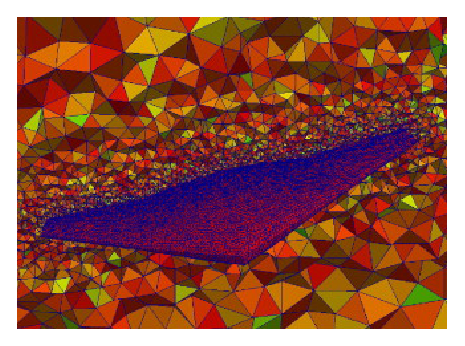
\includegraphics[width=0.44\textwidth]{Fig/mesh_def0}
%    \hspace{3mm}
%    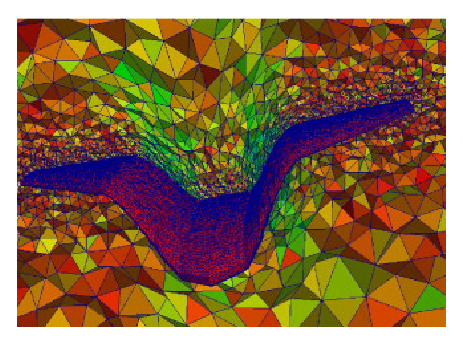
\includegraphics[width=0.44\textwidth]{Fig/mesh_def1}
%  \end{figure}
%\end{frame}

%------------------------------------------------------------------------------

%\begin{frame}
%  \frametitle{CFD solver II: non conforming grid approach}
%
%  \begin{block}{Immersed boundary CFD approach}
%    \begin{itemize}
%    \item Volume mesh does not conform to the surface mesh
%    \item Fixed volume mesh and decoupled geometry surface deformation 
%    \item Fast and robust mesh generation for geometry of arbitrary complexity
%    \item High level of automatization and flexible geometry modeling
%    \item Coupling between volume and surface discretization 
%      \begin{itemize}
%      \item Geometry intersector: can be fast, robust and accurate (CS)
%      \item IB numerical treatment: can be slow, not robust and not accurate (CFD)
%      \end{itemize}
%    \end{itemize}
%  \end{block}
%  \begin{figure}
%    \centering
%    \includegraphics[width=0.65\textwidth]{Fig/embopt}
%  \end{figure}
%
%\end{frame}

%------------------------------------------------------------------------------

%------------------------------------------------------------------------------

\begin{frame}
  \frametitle{IB with the FIVER approach: original formulation}
  \vspace{-2mm}
  \begin{itemize}
  \item Identify immersed boundaries with control volume interfaces $\mathcal{C}_{ij}$
    \begin{figure}[t!]
      \centering
      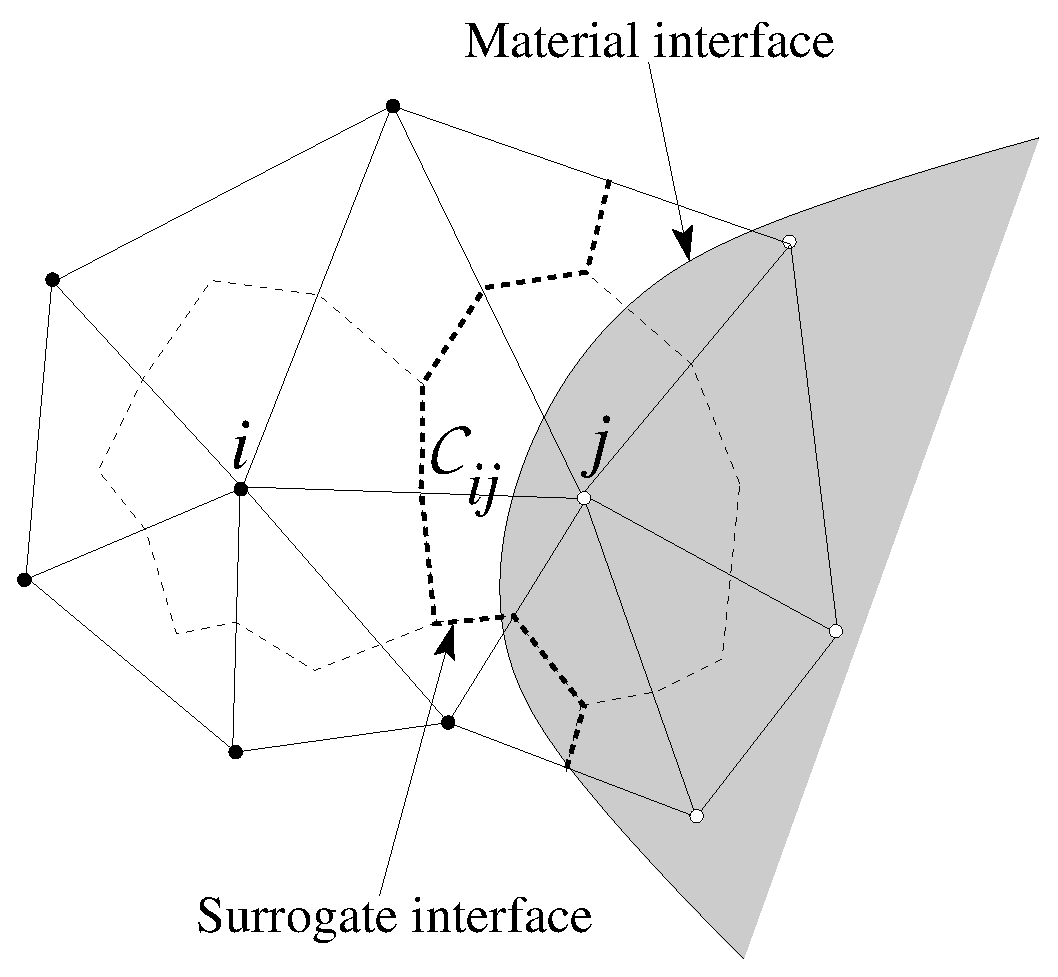
\includegraphics[width=0.35\textwidth]{Fig/fiver1}
    \end{figure} 
    \vspace{-1mm}
  \item Solve exactly local one-dimensional half-Riemann problems at $\mathcal{C}_{ij}$
    \vspace{-2mm}
    \begin{columns}
      \hspace{4mm}
      \begin{column}{0.55\textwidth}
        \begin{equation*}
          \left\{\!\!\!\! \begin{array}{ll}
            \dfrac{\partial \tilde\wbold^\star}{\partial \tau} + \dfrac{\partial\tilde\fbold(\tilde\wbold^\star)}{\partial \xi} = 0 \\[2mm]
            \tilde\wbold^\star(\xi, 0) = \tilde\wbold_{ij}, & \!\!\xi \le 0  \\[2mm]
            \vel(0, \tau)\cdot \nbold_\wall = \vel_\wall\cdot \nbold_\wall, & \!\!0 \le \tau \le \Delta t
          \end{array} \right.
        \end{equation*}
      \end{column}
      \begin{column}{0.43\textwidth}
        \begin{figure}[b!]
          \centering
          \hspace{-5mm}
          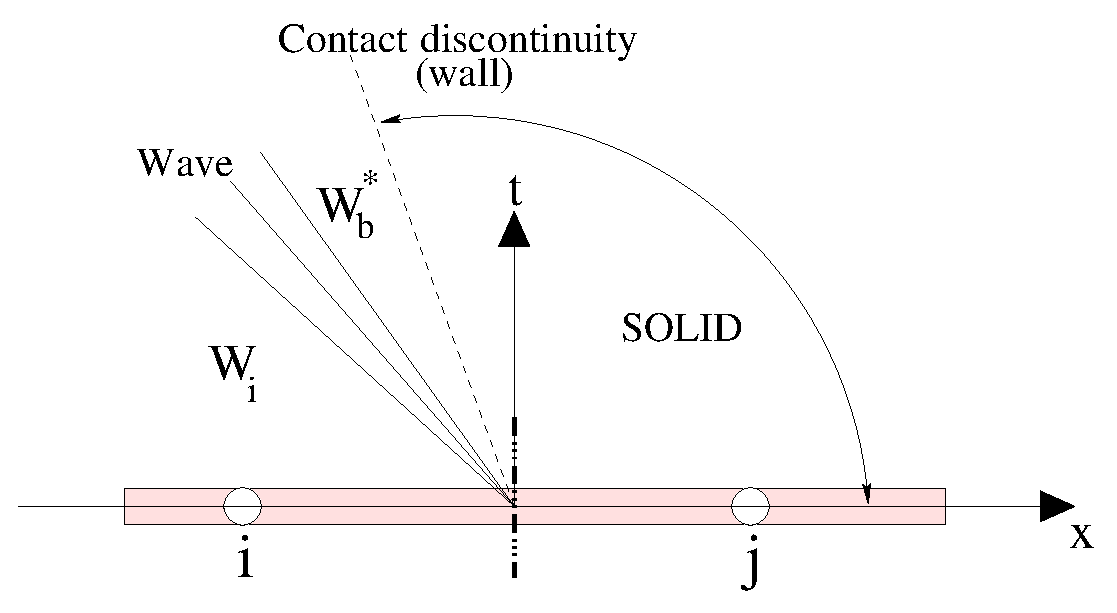
\includegraphics[width=0.99\textwidth]{Fig/riemann}
        \end{figure}
      \end{column}
    \end{columns}
    \item Evaluate numerical flux: $\Fbold_{ij} = \Fbold_{ij}(\wbold_{ij}, \wbold^\star_{b}, \n_{ij})$
  \end{itemize}
\end{frame}

%------------------------------------------------------------------------------

\begin{frame}
  \frametitle{IB with the FIVER approach: enhanced formulation}
  \begin{figure}[h!]
    \centering
    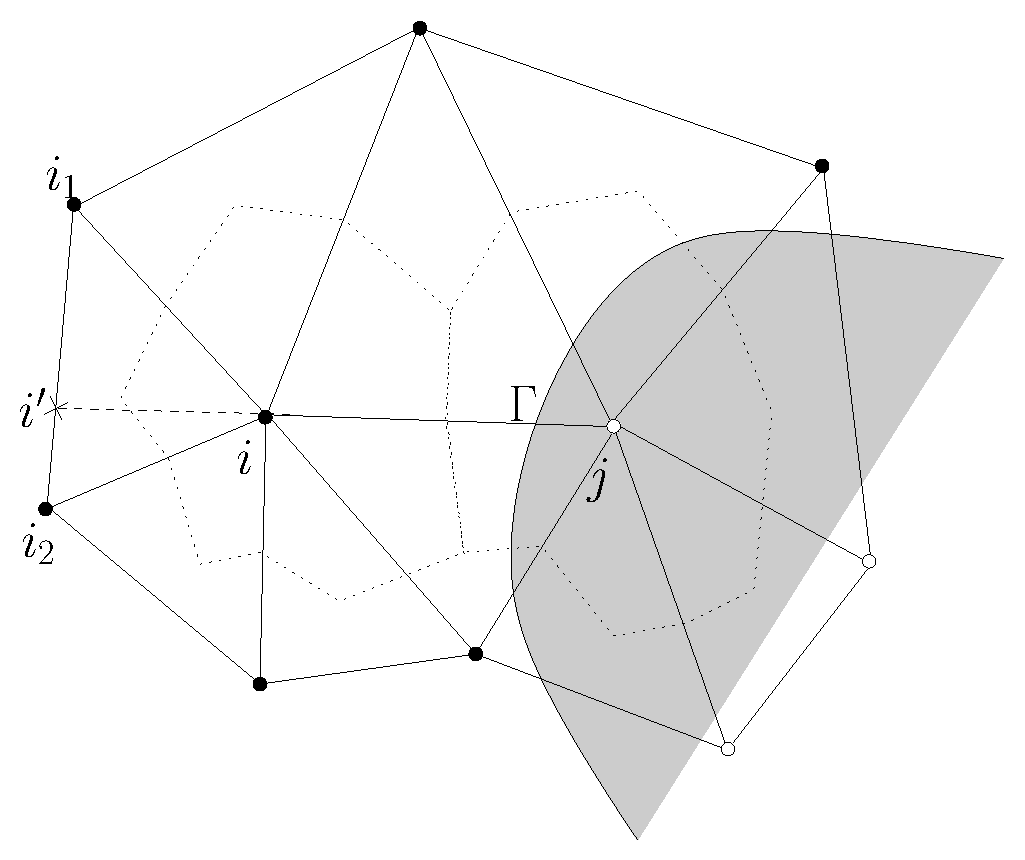
\includegraphics[width=0.35\textwidth]{Fig/fiver2}
  \end{figure}
  \vspace{-5mm}
  \begin{itemize}
  \item The fluid state is extrapolated to the material interface $\Gamma$ \\[-4mm]
    \begin{equation*}
      \wbold_\Gamma = \wbold_i + \nabla \wbold_i \boldsymbol\!\cdot (\xbold_\Gamma - \xbold_i)
    \end{equation*} 
  \item The one-dimensional half-Riemann problem is solved at material interface $\Gamma$\\[-4mm]
    \begin{equation*}
      \tilde\wbold^\star_\Gamma =\tilde\wbold^\star(\tilde\wbold_\Gamma, \vel_\wall, \nbold_\wall)
    \end{equation*} 
  \item The fluid state is inter/extra-polated at control volume interface $\mathcal{C}_{ij}$\\[-4mm]
    \begin{equation*}
      \wbold^\star_{ij} = \wbold^\star_{ij}(\wbold^\star_\Gamma, \wbold_{i'})
    \end{equation*}
  \item Numerical flux at the control volume interface: $\Fbold_{ij} = \Fbold_{ij}(\wbold_{ij}, \wbold^\star_{ij}, \n_{ij})$
  \item  Second-order convergence is recovered in the vicinity of the interface
  \end{itemize}
\end{frame}


%------------------------------------------------------------------------------



\documentclass[../main.tex]{subfiles}
%\usepackage{algorithm}
%\usepackage{algorithmic}
\everymath{\displaystyle}
\def\arraystretch{2.0}
\begin{document}
\setlength{\delimitershortfall}{0pt}
\section{Optimization}\label{sec:optimization}



%\subsection{Basics}\label{sec:basics}

A generic, aeroelastic optimization problem can be written as
\begin{align}
\optcrit(\absvars,\structdisp,\fstate)
&\begin{cases}
&\underset{\absvars}{\text{min }}\costfunc(\absvars) \\%TODO subscribt s
&\eqctr(\absvar)=\vec{0},~~~\eqctr \in \mathbb{R}^{\numeqctr} \\
&\neqctr(\absvar)>\vec{0},~~~\neqctr \in \mathbb{R}^{\numneqctr} \\
\end{cases} \label{eq:generic_optimization_problem_1}\\
&\absvars = \{ \absvars \in \mathbb{R}^{n_{\absvars}} | \absvars_L \leq \absvars \leq \absvars_U \}\label{eq:generic_optimization_problem_2}
\end{align}
Here,  $\costfunc$ is an arbitrary cost function that should be minimized. Note that a maximization problem can easily be obtained by multiplying the cost function by a factor of $-1$. In aerodynamics, a typical example for a cost function would be the \ac{LDR} ratio of an airfoil. The cost-function is described in terms of so-called \textit{abstract variables}. These can have some physical interpretation, but don't necessarily have to(see Section~\ref{sec:design_model}). Since typically, these optimization problems have no finite solution on an unbounded domain, some restrictions/conditions are introduced. In the airfoil example, we would probably specify a minimum lift that is required to support the configuration. Also a maximum stress for the structure will likely have to be specified. These are classical examples of non-equality constraints, denoted by $\neqctr(\absvars)$ in the above formulation. Constraints can also be formulated in an equality sense, for instance geometrical restrictions due to the turbine suspensions.\\
Furthermore, the abstract optimization variables $\absvars$ themselves are typically restricted by lower($\absvars_L$) and upper($\absvars_U$) bounds.\\
The combinations of objective function~$\costfunc$ and constraints $\eqctr$ and $\neqctr$ is typically denoted as optimization criteria $\optcrit$.
\begin{align}\label{eq:optimization_criteria}
&\optcrit=\optcrit(\absvars,\structdisp,\fstate) \nonumber \\
&\structdisp=\structdisp(\absvars),~~~\fstate=\fstate(\absvars)
\end{align}
This thesis follows the \expression{nested analysis and design approach}, meaning that we assume that $\structdisp$ and $\fstate$ always satisfy the aeroelastic state equations. This means that the state equations are not included in the set of constraints, but the structural displacements $\structdisp$ and the fluid state variables $\fstate$ are determined in each iteration.

As \cite{Maute2001} write, the aeroelastic optimization problem can typically be solved by combining three different numerical approaches:
\begin{itemize}
\item Optimization Model
\item Design Model
\item Analysis Model
\end{itemize}

The optimization model describes the solution of the generic optimization problem\eqref{eq:generic_optimization_problem_1}-\eqref{eq:generic_optimization_problem_2}. For this thesis, a \ac{SQP} has been chosen~\cite{Bonnans2006}.\\
The design model links abstract optimization variables~$\absvars$ to actual shapes, structures, geometries or aerodynamics design parameters. For this purpose SDESIGN, a programm specifically written for \ac{SA} purpose in the \ac{FRG}, has been used during this thesis. Its basic concepts an ideas are described in \cite{Maute2003}.\\
Finally, the analysis model provides concepts of evaluation the optimization criteria. Typically, the optimization criteria depend on $\structdisp$ and $\fstate$ which is why a coupled system of equations has to be solved in every design optimization process. The Sensitivity Analysis (SA) is also part of this model. Aeroelastic analysis and Sensitivity analysis are discussed in Section~\ref{sec:aeroelastic_sa}.

\subsection{Optimization Model}\label{sec:optimization_model}
Optimization problems are typically solved by gradient-based methods. The methods are divided into
\begin{itemize}
\item Primal
\item Dual
\item Penalty-barrier   and
\item Lagrange approaches
\end{itemize}
This thesis focuses on Lagrange approaches. For a thorough analysis and comparison of the different approaches, the interested reader is referred to~\cite{Schittkowski1994}.\\
The Lagrangian approach formulates the optimization problem\eqref{eq:generic_optimization_problem_1}\eqref{eq:generic_optimization_problem_2} as an extreme value problem of the Lagrangian:
\begin{align}\label{eq:lagrangian_of_optimization}
\Lagfunc(\absvars,\lagmultseq,\lagmultsneq)=\costfunc(\absvars))=\T{\lagmultseq} \eqctr(\absvars) + \T{\lagmultsneq}\neqctr(\absvars) \\
\end{align}
Here, $\lagmultseq$ denote the Lagrange multipliers for the equality constraints and $\lagmultsneq$ the Lagrange multipliers for the non-equality constraints.
In fact, one can easily see that the original optimization problem can be obtained as saddle point of the Lagrangian:
\begin{align}\label{eq:saddlepoint_optimization}
\pdfrac{\Lagfunc}{\absvars}&=\pdfrac{\costfunc}{\absvars}=\T{\lagmultseq}\pdfrac{\eqctr}{\absvars}+\T{\lagmultsneq}\pdfrac{\neqctr}{\absvars} \\
\pdfrac{\Lagfunc}{\lagmultseq}&=\eqctr=\vec{0} \\
\pdfrac{\Lagfunc}{\lagmultsneq}&=\T{\lagmultsneq}\neqctr=\vec{0}
\end{align}
The \ac{SQP} method, mention before uses a Newton-Rhapsodon algorithm to solve the above system.



\def\incrabsvars{\Delta \absvars}
\def\incrlagmultsneq{\Delta \lagmultsneq}
\def\incrlagmultseq{\Delta \lagmultseq}

\def\PPLagfuncBYabsvars{\ppdfrac{\Lagfunc}{\absvars}}
\def\PLagfuncBYabsvars{\pdfrac{\Lagfunc}{\absvars}}
\def\PneqctrBYabsvars{\pdfrac{\neqctr}{\absvar}}
\def\PeqctrBYabsvars{\pdfrac{\eqctr}{\absvar}}

\begin{align}\label{eq:saddlepoint_newtonform}
\begin{bmatrix}
\it{\PPLagfuncBYabsvars}                & \it{\PneqctrBYabsvars} & \it{\PeqctrBYabsvars} \\
\it{\lagmultsneq}\it{\PneqctrBYabsvars} & \it{\eqctr}            & \vec{0}               \\
\it{\PeqctrBYabsvars}                   & \vec{0}                & \vec{0}
\end{bmatrix}
	\begin{bmatrix}
	\incrabsvars \\
	\incrlagmultsneq \\
	\incrlagmultseq
	\end{bmatrix}\
	=
    -\begin{bmatrix}
		\it{\PLagfuncBYabsvars} \\
		\T{\it{\lagmultsneq}} \it{\neqctr} \\
		\it{\eqctr}
		\end{bmatrix}
\end{align}
Here $\it{(\cdot)}$ denotes the iteration index of the optimization loop.\\
~\\
The linear Equations~\eqref{eq:saddlepoint_newtonform} can also be formulated as an equivalent quadratic minimization problem:



\begin{align}
\underset{\absvars}{\text{min }}( \frac{1}{2} \T{\incrabsvars} \it{\PPLagfuncBYabsvars} \incrabsvars + \frac{\partial \it{\costfunc}}{\partial \absvars} ) \label{eq:quadratic_minimization_problem_1}\\
\it{\PneqctrBYabsvars} \incrabsvars+\it{\neqctr} \geq \vec{0} \label{eq:quadratic_minimization_problem_2}\\
\it{\PeqctrBYabsvars} \incrabsvars+\it{\eqctr} = \vec{0} \label{eq:quadratic_minimization_problem_3}
\end{align}
\\
In the above formulation, the evaluation of the second derivative of the Lagrangian(Hessian of $\Lagfunc$) is the numerically most expensive part. Usually it is preferred to approximate it by a first-order information, for example by the \ac{DFP} or by the \ac{BFGS} method. However, this simplification introduces an error that one should be aware of. Some correction methods have been proposed trying to minimize the error. In this thesis we adapt the one proposed by~\cite{Maute2001}:
\begin{align}\label{eq:correction_step}
\begin{bmatrix}
\absvars^{(k+1)} \\
\lagmultseq^{(k+1)} \\
\lagmultsneq^{(k+1)}
\end{bmatrix} =
  \begin{bmatrix}
  \it{\absvars} \\
  \it{\lagmultseq} \\
  \it{\lagmultsneq} \\
  \end{bmatrix} +
    \it{\alpha}
    \begin{bmatrix}
    \it{\incrabsvars} \\
    \it{\incrlagmultseq} \\
    \it{\incrlagmultsneq} \\
    \end{bmatrix}
\end{align}
The appropriate step size $\it{\alpha}$ is determined by a line search. AS~\cite{Maute2001} write, due to this insufficiencies, the Lagrangian can not be used to measure an improvement. Instead, a merit function is introduced that is minimized by the line-search. A local minimum is reached by following a sequence of decreasing merit function values. Convergence of the process can be measured via the $\mathcal{L}_2$-norm of the residual of the Kuhn-Tucker conditions\eqref{eq:saddlepoint_optimization}.\\
By construction, the constraints are satisfied only when the optimum point is reached.



%
\subsection{Design Model}\label{sec:design_model}
The design model represent the essential link between the described optimization model and the analysis model. Generally speaking, it relates physical design parameters to abstract ones.
\begin{align}
\physvars=\physvars(\absvars),~~~\physvars \in \mathbb{R}^{n_{\physvars}} \label{eq:physvarsTOabsvars}
\end{align}
Here, $n_{\physvars}$ denotes the number of physical design parameters.
To define a relation between the abstract optimization variables and the motion of the nodes, the following design model is introduced:
\begin{align}
\mms=\mms(\absvars)
\end{align}

As~\cite{Maute2001} explain, it is unpractical to identify an abstract variable directly with an increment of the coordinate of a grid point. Instead, two approaches, namely geometrical and mechanical can be adopted for constructing the generic design model.
\paragraph{Mechanical approach}
In the mechanical approach, the shape variation is identified with a superposition of fictitious structural deformations $\fic{\structdisp}_{j}$ due to fictitious loads $\mu \fic{\vec{P}}_{j}$ and fictions support conditions
\begin{align}
\mms=\sum_j \fic{\structdisp}_j = \sum_j \inv{\fic{\stiffmat}_j} \mu_j \fic{\vec{P}}_{j} \label{eq:mechanical_approach}
\end{align}
where $\fic{\stiffmat}_j$ is a fictitious pseudo structure stiffness matrix representing the fluid domain compatible to the current fictions support conditions.

\paragraph{Geometrical approach}
The geometrical approach describes the geometry of the structure or the fluid boundary the design element concept. Here, the shape of a body $\tensor{X}$ is approximated by so-called design elements as follows:
\begin{align}
\tensor{X}=\sum_{j} \phi_{j}(\xi) \hat{\tensor{X}}_j \label{eq:geometrical_approach}
\end{align}
Here, $\phi_{j}(\xi)$ is a shape function, $\hat{\tensor{X}}_j$ is the vector of control nodes and $\xi$ represents the reference coordinate. In the design element concept, the variation of the control nodes of the design element is used to vary the shape of the body. The variation of the control nodes position denoted as "mesh-motion" is given as $\mms=\Delta \hat{\tensor{X}} $
\begin{align}
\mms = \sum_j \phi_{j}(\xi) \hat{\mms}_j \label{eq:mms}
\end{align}

Just as in Finite Elements, where the shape-functions can not only be used to describe the solution field, but also the body's geometry and material parameters, the design element concept can be applied to prescribe parameter distributions and their variations in the optimization process. A simple sketch of the concept is provided in Figure~\ref{fig:sketch_geometrical_approach}
\\
Both approaches have pros and cons, that are quickly discussed in \cite{Maute2003}, this thesis utilizes the geometrical approach solemnly.

\begin{figure}[h!]
	\begin{center}
        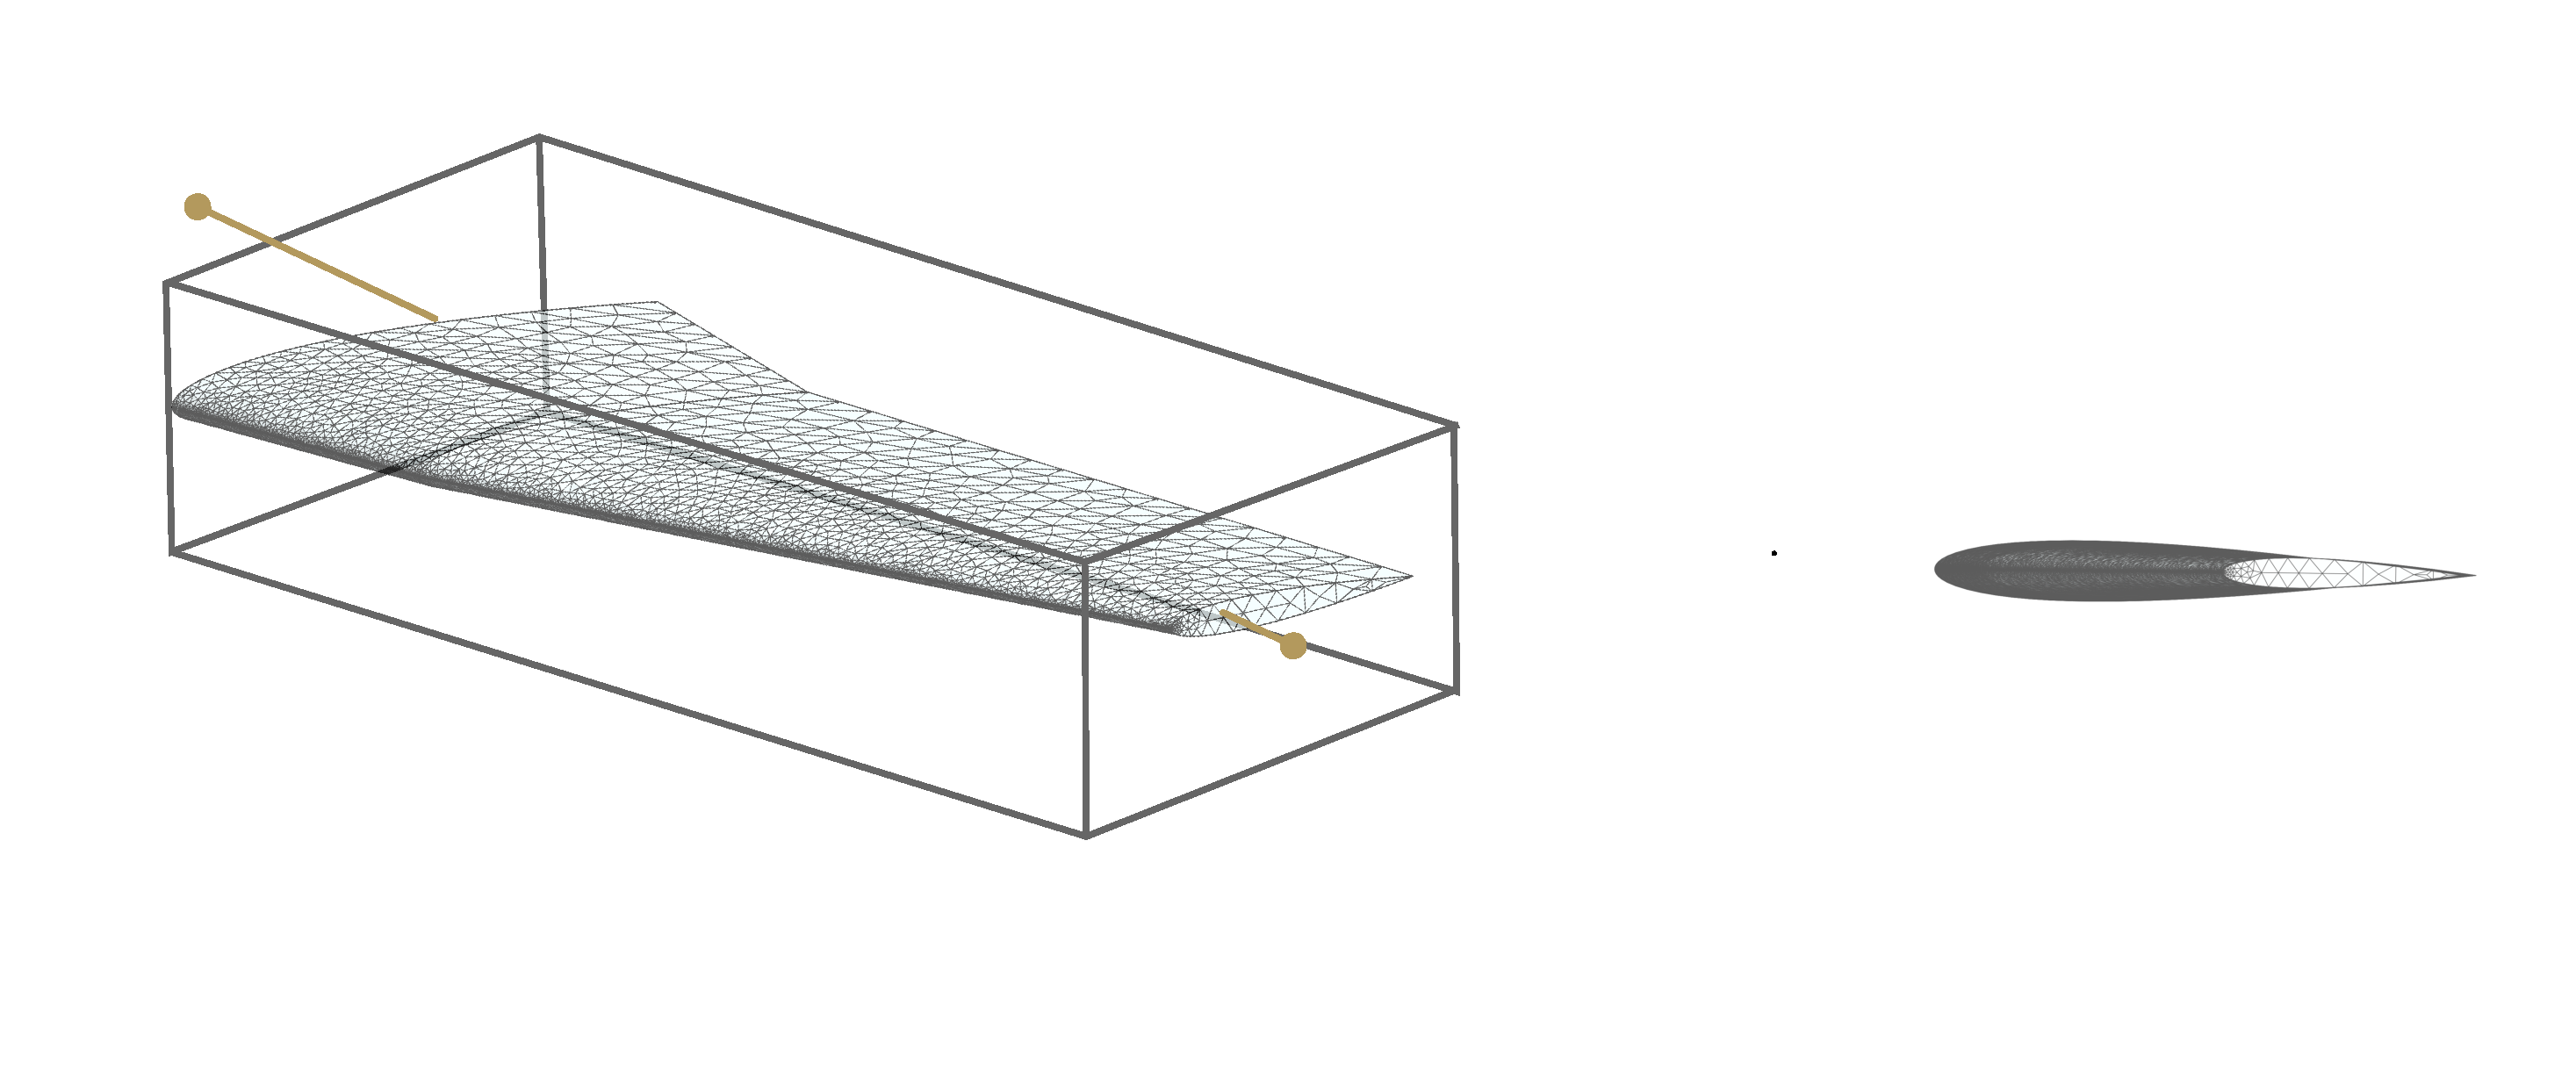
\includegraphics[width=1.0\textwidth]{\mainpath/fig/pdf/sdesign.pdf}
        \caption[Design-model: geometrical approach]{Geometrical approach for the design model as explained in Section~\ref{sec:design_model}. A NACA type airfoil is considered here as an example. The airfoil is embedded in a bounding box defined by eight so-called control nodes. The position of these control nodes can be varied, which alternates the shape of the airfoil according to some interpolation functions defined on the nodes. The 24 displacement unknowns are denoted as "abstract shape parameters". Abstract shape variables can be arbitrarily defined. As an example, a rotation axis is defined through the wing.}
		\label{fig:sketch_geometrical_approach}
    \end{center}
\end{figure}

\begin{figure}[h!]
	\begin{center}
        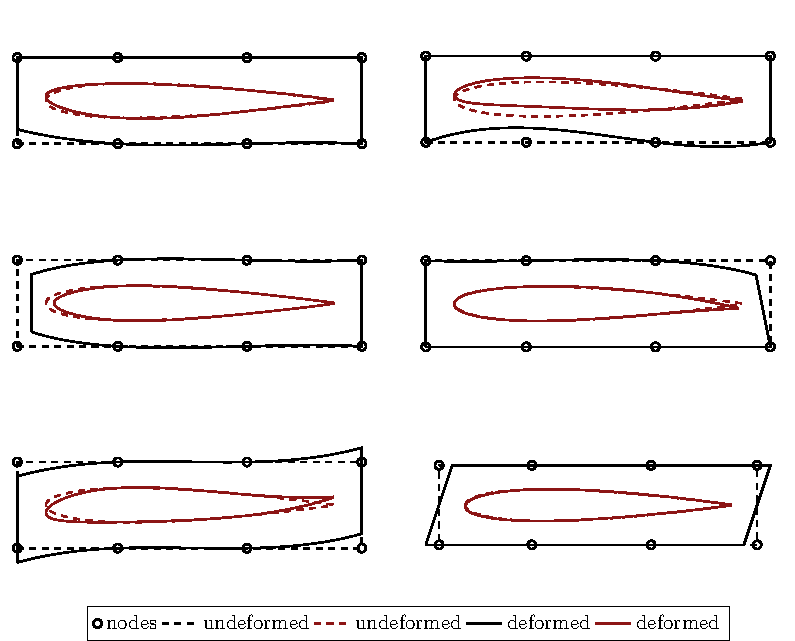
\includegraphics{\mainpath/fig/tikz/build/sdesign_visualization.pdf}
        \caption[Design element visualization]{Visualization of the design element concept, exemplarily shown on a NACA0012 airfoil. For simplicity, a single design element(cubic in the horizontal direction and linear in the vertical direction) is used. Both the initial configuration(dashed lines) and the deformed configuration(full lines) are plotted. Although only eight design element nodes are provided, the function space of the design element allows for a great variation of the airfoil shape. Also, the size of the parameter space is now independent of the airfoil mesh size. From this perspective, the design element concept can be regarded as an model reduction for the shape variation.}
		\label{designelement_concept_2D}
    \end{center}
\end{figure}

%TODO talk about SDESIGN
\subsection{Analysis Model}\label{sec:analysis_model}
In the analysis model, the optimization criteria $\optcrit$ are determined for a given set of obtimization variables $\absvar$. Since the optimization algorithm choses in this thesis is based on gradients, the gradients of the optimization criteria with respect to the abstract variables are determined in this step. A main focus on this thesis has been the appropriate evaluation of these derivatives, we therfore denote the subsequent chapter~\ref{sec:SA} to the issue.

\end{document}

\documentclass[../main.tex]{subfiles}
%\usepackage{algorithm}
%\usepackage{algorithmic}
\everymath{\displaystyle}
\def\arraystretch{2.0}
\begin{document}
\setlength{\delimitershortfall}{0pt}

\def\incrabsvars{\Delta \absvars}
\def\incrlagmultsneq{\Delta \lagmultsneq}
\def\incrlagmultseq{\Delta \lagmultseq}

\def\PPLagfuncBYabsvars{\ppdfrac{\Lagfunc}{\absvars}}
\def\PLagfuncBYabsvars{\pdfrac{\Lagfunc}{\absvars}}
\def\PneqctrBYabsvars{\pdfrac{\neqctr}{\absvar}}
\def\PeqctrBYabsvars{\pdfrac{\eqctr}{\absvar}}

\def\DoptcritJBYabsvarI{\frac{d \optcrit_{j}}{d \absvar_{i}}}
\def\PoptcritJBYabsvarI{\pdfrac{\optcrit_{j}}{\absvar_{i}}}

\def\PoptcritJBYstructdisp{\pdfrac{\optcrit_{j}}{\structdisp}}
\def\PoptcritJBYmms       {\pdfrac{\optcrit_{j}}{\mms}}
\def\PoptcritJBYfstate    {\pdfrac{\optcrit_{j}}{\fstate}}

\def\DoptcritJBYstructdisp{\tfrac{\optcrit_{j}}{\structdisp}}
\def\DoptcritJBYmms       {\tfrac{\optcrit_{j}}{\mms}}
\def\DoptcritJBYfstate    {\tfrac{\optcrit_{j}}{\fstate}}

\def\DstructdispBYabsvarI{\frac{d \structdisp}{d \absvar_{i}} }
\def\DmmsBYabsvarI       {\frac{d \mms       }{d \absvar_{i}} }
\def\DfstateBYabsvarI    {\frac{d \fstate    }{d \absvar_{i}} }

\def\PstructdispBYabsvarI{\pdfrac{d \structdisp}{d \absvar_{i}} }
\def\PmmsBYabsvarI       {\pdfrac{d \mms       }{d \absvar_{i}} }
\def\PfstateBYabsvarI    {\pdfrac{d \fstate    }{d \absvar_{i}} }

\def\PEOSstructBYabsvarI{\pdfrac{\EOSstruct} {\absvar_i}}
\def\PEOSmeshBYabsvarI  {\pdfrac{\EOSmesh}  {\absvar_i}}
   %\def\PEOSfluidBYabsvarI{\pdfrac{\EOSfluid}{\absvar_i}}

\def\DEOSstructBYabsvarI{\tfrac{\EOSstruct} {\absvar_i}}
\def\DEOSmeshBYabsvarI  {\tfrac{\EOSmesh}  {\absvar_i}}
  %\def\DEOSfluidBYabsvarI{\tfrac{\EOSfluid}{\absvar_i}}

\def\PEOSstructBYstructdisp{\pdfrac{\EOSstruct} {\structdisp}}
\def\PEOSstructBYmms{\pdfrac{\EOSstruct}{\mms}}
\def\PEOSstructBYfstate    {\pdfrac{\EOSstruct}{\fstate}}

\def\PEOSmeshBYstructdisp{\pdfrac{\EOSmesh}{\structdisp}}
\def\PEOSmeshBYmms       {\pdfrac{\EOSmesh} {\mms}}
\def\PEOSmeshBYfstate    {\vec{0}}

\def\PEOSfluidBYstructdisp{\vec{0}}
   %\def\PEOSfluidBYmms       {\pdfrac{\EOSfluid} {\mms}}
   %\def\PEOSfluidBYfstate    {\pdfrac{\EOSfluid} {\fstate}}

\def\PstructdispBYabsvarI{\pdfrac{\structdisp} {\absvar_i}}
\def\PmmsBYabsvarI       {\pdfrac{\mms}        {\absvar_i}}
\def\PfstateBYabsvarI    {\pdfrac{\fstate}     {\absvar_i}}



\chapter{Fluid \acf{SA}}\label{sec:SA}
\addcontentsline{lof}{chapter}{Fluid \acf{SA}}
As explained in chapter \ref{sec:optimization}, optimization is based on the calculations of gradients, also denoted as \acf{SA}.

\subsection{Connection between discretization and differentiation}\label{sec:discretization_vs_differentiation}
When it comes to calculating the gradients of a solution of a PDE, there are two fundamentally different approaches one could take.\\
Firstly one could think of first deriving the continous equation and then applying the discretization scheme. On the other hand its equaly legitimate to first apply the discretization and compute the gradients of that, approximated solution. This thesis focuses uses the latter one, the reasons being explained in Figure~\ref{fig:discretization_differentiation_sequence}.


 \begin{figure}[h!]
	\begin{center}
        \includegraphics{\mainpath/fig/tikz/build/discretization_differentiation_sequence.pdf}
        \caption[Sensitivity Analysis approaches]{Two different approaches of \ac{SA}. The question here is whether to discretize the system of equations first and then compute the derivatives of the approximate solution, or whether the continuous system of equation is first derived and discretized afterwards. Both approaches are valid, the final result however will generally not be the same. We have solemnly focused on the case of derivation after discretization in this thesis(thick lines). There are several reason to this. Firstly, if one chose to first derive and then compute a discretized solution, one would solve a completely different equation. If on the other hand the discretization(e.g. Finite Volumes) is done first, standard solvers can be utilized. What is more, approximating the derivative by a Finite difference becomes much easier, since the finite difference evaluation involves only a evaluation of $\dmat{F}$, which a standard fluid solver is perfectly capable of, whereas the \ac{FD} approximation in the other case would involve evaluations of the continuous function and the discretization of the obtained expression which would be much more cumbersome. \textbf{Think about whether this is correct} }
		\label{fig:discretization_differentiation_sequence}
    \end{center}
\end{figure}





\subsection{Sensitivity derivation}
When it comes to \ac{SA} within the context of \ac{CFD}, one also has to distinguish between \ac{SA} of the non-coupled fluid problem and the \ac{SA} in the fully coupled aeroelastic case. The latter case is much more involved, since it requires additional terms from the Structure and mesh motion equations. In the following we will therefore begin with the \ac{SA} of a regular fluid problem. A generalization to a coupled FSI problem will follow.
 \\


As mentioned in Section~\ref{sec:optimization}, we typically deal with an optimization criteria $\optcrit_j$, that is in this case dependent on the fluid state variables $\fstate$ that themselves may depend on abstract variables $\absvar_i$
\begin{align}
\optcrit_j=\optcrit_j(\fstate(\absvar_i))
\end{align}



\begin{align}\label{eq:sensitivity_startingpoint}
\DoptcritJBYabsvarI\bigg\rvert_{\fstate_0}=
\underbrace{\PoptcritJBYabsvarI\bigg\rvert_{\fstate_0}}_{
                                                        \substack{
                                                                 \text{\hltblue{directy derived from}} \\
                                                                 \text{\hltblue{the definition of} $\optcrit$}
                                                                 } 
                                                        }  +
\underbrace{\PoptcritJBYfstate\bigg\rvert_{\fstate_0}}_ {
                                                        \substack{
                                                                 \text{\hltgreen{derived analytically or~~}}\\
                                                                 \text{\hltgreen{by} \ac{FD}}
                                                                 }
                                                        }
\underbrace{\DfstateBYabsvarI\bigg\rvert_{\fstate_0}}_  {
                                                        \substack{
                                                                 \text{\hltyellow{derived from dynamic}}\\
                                                                 \text{\hltyellow{fluid equilibrium}}
                                                                 }
                                                        }
\end{align}
\subsubsection{Calculation of $\PoptcritJBYabsvarI\bigg\rvert_{\fstate_0}$}
In this thesis, we restrict ourselves to Lift($L$), Drag($D$) and combinations of  these quantities( e.g. Lift-Drag ration $\frac{L}{D}$ ) as optimization criteria $\optcrit$. As abstract variables we only consider the free stream mach-number $\machnum_{\infty}$, the free-stream angle of attack $\aoa$ and an airfoil shape parameter as explained in chapter \ref{sec:design_model}.
The formula for the lift over an airfoil can be written as


If $\Gamma_{FS}$ denotes the fluid structure interface, which in the \ac{ALE} context coincides with the airfoil surface, one can formulate the lift and drag of an airfoil in a steady state as:
\begin{align}\label{eq:lift_and_drag_integrals}
\lift=\int_{\Gamma_{FS}} p(\fstate,\cvec{x}) \normal(\cvec{x})\cdot \cvec{e}_L dS \nonumber\\
\drag=\int_{\Gamma_{FS}} p(\fstate,\cvec{x}) \normal(\cvec{x})\cdot \cvec{e}_D dS \\
\end{align}
where $\cvec{e}_D$ is the unit vector pointing in the direction of the free stream, and $\cvec{e}_L$ is the unit vector perpendicular to that.
We therefor note, that $\pdfrac{\lift}{\absvar_i}$ and $\pdfrac{\drag}{\absvar_i}$ are zero for $\absvar_{i}=\machnum_{\infty}$ and $\absvar_{i}s=\aoa$ and non-zero if $\absvar_{i}$ is a shape parameter.\\
Also, having determined the derivatives $\pdfrac{\lift}{\absvar_i}$ and $\pdfrac{\drag}{\absvar_i}$, the derivative of the Lift-Drag ratio follows simply as
\begin{align}\label{eq:lifttoddrag_by_absvar}
-\pdfrac{(\frac{\lift}{\drag})}{\absvar_i}\rvert_{\fstate_0}=
-\frac{\drag_0 \pdfrac{\lift}{\absvar_i}\rvert_{\fstate_0} - \lift_0 \pdfrac{\drag}{\absvar_i}\rvert_{\fstate_0} }{{\drag_0}^2}
\end{align}


\subsubsection{Calculation of $\PoptcritJBYfstate\bigg\rvert_{\fstate_0}$}
The derivative of the optimization criteria with respect to the fluid state vector can again be splitted into Lift and Drag part.
For an aeroelastic simulations, the biggest difficulty here is the dependence on the fluid state by the fluid-srtucture interface itself.
We are therefore faced with a derivative of an integral quantity, where the integration area itself is dependent on the quantiti of interest.\\
For this purpose, we recall the leibnitz rule from calculus:
\begin{align}\label{eq:leibnitz_rule}
\frac{d}{dx}\Big(\int_{a(x)}^{b(x)} f(x,t) dt \Big) =
f(x,b(x))\cdot \frac{d}{dx}b(x)-
f(x,a(x))\cdot \frac{d}{dx}a(x)+
\int_{a(x)}^{b(x)} \frac{d}{dx} f(x,t) dt
\end{align}

Alternatively, we can directly switch to the discrete form, where the calculation of Lift and drag as outlined in Equation~\eqref{eq:lift_and_drag_integrals} can be performed as
\begin{align}\label{eq:discrete_lift_and_drag_formulas}
L=\sum_{e \in \sum_{\Gamma_{FS}}} \sum_{i=1}^{n_g} g_i \dpres(\dfstate_i,\dmpos_i) \normal_e \cdot e_L
D=\sum_{e \in \sum_{\Gamma_{FS}}} \sum_{i=1}^{n_g} g_i \dpres(\dfstate_i,\dmpos_i) \normal_e \cdot e_D
\end{align}
where $\sum_{\Gamma_{FS}}$ is the set of surface elements on the fluid-structure interface, $n_g$ is the number of gauss-points and $g_i$ are the gauss weights. The dependency of the surface shape, on the fluid state vector is now reflected in non-zero derivatives of the gauss point locations.

Finally, the derivative of the lift-to-drag ratio can be obtained analogously to equation~\eqref{eq:lifttoddrag_by_absvar} as
\begin{align}\label{eq:lifttodrag_by_dfstate}
\pdfrac{(\frac{\mathsf{L}}{\mathsf{D}})}{\dfstate}\rvert_{\fstate_0}=
\frac{\mathsf{D}_0 \pdfrac{\mathsf{L}}{\dfstate}\rvert_{\fstate_0} - \mathsf{L}_0 \pdfrac{\drag}{\dfstate}\rvert_{\dfstate_0} }{{\mathsf{D}_0}^2}
\end{align}


\subsubsection{Calculation of $\DfstateBYabsvarI\bigg\rvert_{\fstate_0}$}

Also, we keep in mind, that the state equation of the fluid can be expressed as
\begin{align}
\EOSfluid(\fstate(\absvar_i),\mms(\absvar_i),\absvar_i)=
\pdfrac{\fstate(\absvar_i)}{t}+\nabla\cdot\fluxesconv(\fstate(\absvar_i))+\nabla\fluxesdiff(\fstate(\absvar_i))+S=
\vec{0}
\end{align}

After discretization, we have derived our discrete governing equation as 
\begin{align}\label{eq:nse_final_discretized_2}
\pdfrac{\bar{\dfstate_i}}{t} +
\sum_{j \in \vertexset(i)} \fluxesnum_{ij}(\dfstate_{ij},\dfstate_{ji},\wnormal_{ij}) -
\sum_{T_i \in \elementset(i)} \int_{T_j} \difftensor \nabla \dfstate \nabla \phi_j dx =
\vec{0}
\end{align}
For the pupose of Sensitivity analysis around a given steady state, the fluid-state vector does not change in time, and can thus be ommitted, also we summaraize the convective and the diffusivee part as $\dresidual$ 
\begin{align}\label{eq:nse_final_discretized_notationchange}
\cancelto{0}{\pdfrac{\bar{\dfstate_i}}{t}} +
\underbrace{
  \underbrace{\sum_{j \in \vertexset(i)} \fluxesnum_{ij}(\dfstate_{ij},\dfstate_{ji},\wnormal_{ij})}_{\dresidual^i} -
  \underbrace{\sum_{T_i \in \elementset(i)} \int_{T_j} \difftensor \nabla \dfstate \nabla \phi_j dx}_{\dresidual^v}      }_{\dresidual} =
\vec{0}
\end{align}
where $\dresidual^i$ denotes the inviscid residual and $\dresidual^v$ the viscous contribution.
We now can express the steady state equation in very compact form as:
\begin{align}\label{eq:discrete_steady_state}
\dresidual=\dvec{0}
\end{align}


In general, this residual depends on the fluid state solution $\dfstate$ as well as on a potential mesh movement $\dmpos$, both of which can be dependent on the abstract design variable. Additionally, a direct dependence on $\absvar$ might be encountered too.
\begin{align}
\dresidual(\dfstate(\absvar),\dmpos(\absvar),\absvar)=\dvec{0}
\end{align}

The total derivative of the residual with respect to the design variable can thus be expanded via the chain rule to
%\begin{align}
%\DEOSfluidBYabsvarI=\vec{0}=
%\PEOSfluidBYabsvarI+
%\PEOSfluidBYfstate\DfstateBYabsvarI+
%\PEOSfluidBYmms\DmmsBYabsvarI
%\end{align}

\def\DdresidualBYabsvarI{ \tfrac{\dresidual}{\absvar_i} }
\def\PdresidualBYabsvarI{ \pdfrac{\dresidual}{\absvar_i} }
\def\PdresidualBYdfstate{ \pdfrac{\dresidual}{\dfstate}  }
\def\DdfstateBYabsvarI  { \tfrac{\dfstate}{\absvar_i}   }
\def\PdresidualBYdmms   { \pdfrac{\dresidual}{\dmpos}     }
\def\DdmmsBYabsvarI     { \tfrac{\dmpos}{\absvar_i}      }
\begin{align}
\DdresidualBYabsvarI=\vec{0}=
\DdresidualBYabsvarI                      +
\PdresidualBYdfstate    \DdfstateBYabsvarI +
\PdresidualBYdmms       \DdmmsBYabsvarI
\end{align}



Therefore the total derivative of the fluid state with respect to the shape variable, needed in equation \eqref{eq:sensitivity_startingpoint}, can be obtained by solving
\begin{align}\label{eq:dfstate_by_absvarI}
\PdresidualBYdfstate    \hleyellow{\DdfstateBYabsvarI}=
-\DdresidualBYabsvarI 
-\PdresidualBYdmms       \DdmmsBYabsvarI
\end{align}


In this equation, $\PdresidualBYabsvarI$ can be computed analytically or by \ac{FD}.
This part is the most cumbersome part of the whole sensitivity analysis, which is why we denoted a full chapter(\ref{sec:dresidual_derivative}) to it.

The derivative of the mesh motion with respect to the abstract variables is often denoted as "shape gradient". It can be divided into two components:
\begin{itemize}
\item The interface component $\tfrac{\mms_\Gamma}{\absvar_i}$, which is associated with the grid points lying on the fluid boundary
\item The interior component $\tfrac{\mms_\Omega}{\absvar_i}$, which is associated with the grid points located in the interior $\Omega$ of the computational domain.
\end{itemize}
The interface component is determined by the structure. Having obtained this one, the interior component can be computed by solving an auxiliary, fictitious Dirichlet problem:
\begin{align}
\tfrac{\mms_\Omega}{\absvar_i}=-\left[\inv{\fic{\stiffmat}_{\Omega\Omega}} \fic{\stiffmat}_{\Omega\Gamma}\right] \tfrac{\mms_\Gamma}{\absvar_i}
\end{align}
where $\fic{\stiffmat}$ is a pseudo stiffness matrix that can be obtained by a simple spring analogy or similar approaches.
In general, the mesh-motion algorithm should be chosen consistently with the one used in the calculation of the steady state solution.
For the later introduced Embedded framework, $\tfrac{\mms}{\absvar_i}$ is the position vector of the embedded discrete surface
 \\
 
\subsection{Full sensitivity equation}\label{sec:full_sensitivity_equation}
After inserting \eqref{eq:lifttoddrag_by_absvar}, \eqref{eq:lifttodrag_by_dfstate} and \eqref{eq:dfstate_by_absvarI} into \eqref{eq:sensitivity_startingpoint}, one can derive the final sensitivity equations for the special case of a rigid or non-existing structure as
\begin{align}\label{eq:full_sa_nostruct}
\tfrac{\optcrit_j}{\absvar_i}\bigg\rvert_{\dfstate_0} &=
-\tfrac{\optcrit_j}{\fstate}\bigg\rvert_{\dfstate_0}
\inv{\left[\PdresidualBYdfstate\bigg\rvert_{\fstate_0}\right]}
\left(
  \PdresidualBYabsvarI\bigg\rvert_{\fstate_0} +
  \begin{bmatrix}
    \alpha\pdfrac{\dresidual}{\dmms_\Omega}\bigg\rvert_{\dfstate_0}~
    \pdfrac{\dresidual}{\dmms_\Gamma}\bigg\rvert_{\dfstate_0}
  \end{bmatrix}
  \begin{bmatrix}
    \alpha \inv{\fic{\stiffmat}_{\Omega\Omega}} \fic{\stiffmat}_{\Omega\Gamma} \\
    \eye
  \end{bmatrix}
  \tfrac{\dmms_\Gamma}{\absvar_i}
\right)\\
\alpha&=
\begin{cases}
  1\text{  in \ac{ALE} framework}\\
  0\text{  in Embedded framework}
\end{cases}
\end{align}

\pagebreak


\chapter{Aero-elastic \acl{SA}}\label{sec:aeroelastic_sa}
The previous chapter dealt with the \ac{SA} of a pure fluid problem. Boundary, or respectively mesh-movement in general, was only induced due to shape variation via design variables itself. However, one can easily decieve a system, where the fluid interacts with an elastic structure. This would introduce an additional dependency of the structure shape, and thus fluid-structure interface, on the fluid solution. Also, a fully coupled system introduces a direct connection between the stress resultants in the structure with the fluid solutions.\
This chapter therfore investigates the \ac{SA} of such a coupled system of equations. Considerations are build upon the derivations in chapter~\ref{sec:SA} and the coupled three-field \ac{FSI} formulation described in chapter~\ref{sec:3_field_formulation}.\\
The \ac{SA} approach applied in this thesis is based on the work of~\cite{Sobieszczanski1990}, for deriving the \ac{GSE} of coupled systems. As introduced by the authors of\cite{Maute2001}, we utilize the three-field formulation of \cite{Farhat1995}.




The derivative of the optimization criterion~$\optcrit_j$, as introduced in Equation~\eqref{eq:optimization_criteria}, with respect to the optimization variable $\absvar_i$ gives:
\begin{align}
\DoptcritJBYabsvarI &=  \PoptcritJBYabsvarI    +
\PoptcritJBYstructdisp \hleblue{\DstructdispBYabsvarI}  +
\PoptcritJBYmms        \hleblue{\DmmsBYabsvarI}  +
\PoptcritJBYfstate     \hleblue{\DfstateBYabsvarI}
\\
&=
\PoptcritJBYabsvarI+
\T{\begin{bmatrix}
\PoptcritJBYstructdisp \\[0.5em]
\PoptcritJBYmms        \\[0.5em]
\PoptcritJBYfstate     \\[0.5em]
\end{bmatrix}}
\cdot
\begin{bmatrix}
\DstructdispBYabsvarI \\[0.5em]
\DmmsBYabsvarI        \\[0.5em]
\DfstateBYabsvarI     \\[0.5em]
\end{bmatrix}
\end{align}
where the partial derivatives$,\PoptcritJBYstructdisp,\PoptcritJBYmms\text{ and } \PoptcritJBYfstate$ can be directly evaluated within the discretized structure and fluid model through the relation between structural, aerodynamic design and abstract optimization parameters defied in the design model~\ref{sec:design_model}.\\
The cumbersome part are the derivatives $\DstructdispBYabsvarI,\DmmsBYabsvarI\text{~and~}\DfstateBYabsvarI$
To obtain them, the governing equations \eqref{eq:3field_basic}\textbf{TODO write down governing equations} have to be derived:




%Differentiation of the governing equations
\def\PEOSstructBYabsvarI{\pdfrac{\EOSstruct} {\absvar_i}}
\def\PEOSmeshBYabsvarI  {\pdfrac{\EOSmesh}  {\absvar_i}}
\def\PEOSfluidBYabsvarI{\pdfrac{\EOSfluid}{\absvar_i}}

\def\PEOSstructBYstructdisp{\pdfrac{\EOSstruct} {\structdisp}}
\def\PEOSstructBYmms{\pdfrac{\EOSstruct}{\mms}}
\def\PEOSstructBYfstate    {\pdfrac{\EOSstruct}{\fstate}}

\def\PEOSmeshBYstructdisp{\pdfrac{\EOSmesh}{\structdisp}}
\def\PEOSmeshBYmms       {\pdfrac{\EOSmesh} {\mms}}
\def\PEOSmeshBYfstate    {\vec{0}}

\def\PEOSfluidBYstructdisp{\vec{0}}
\def\PEOSfluidBYmms       {\pdfrac{\EOSfluid} {\mms}}
\def\PEOSfluidBYfstate    {\pdfrac{\EOSfluid} {\fstate}}

\def\PstructdispBYabsvarI{\pdfrac{\structdisp} {\absvar_i}}
\def\PmmsBYabsvarI       {\pdfrac{\mms}        {\absvar_i}}
\def\PfstateBYabsvarI    {\pdfrac{\fstate}     {\absvar_i}}

\begin{align}\label{eq:govering_eqautions_derivative}
\def\arraystretch{2.0}
\begin{bmatrix}
\PEOSstructBYabsvarI \\[0.5em]
\PEOSmeshBYabsvarI   \\[0.5em]
\PEOSfluidBYabsvarI
\end{bmatrix} +
  \underbrace{\begin{bmatrix}
  \PEOSstructBYstructdisp & \PEOSstructBYmms & \PEOSstructBYfstate \\[0.5em]
  \PEOSmeshBYstructdisp   & \PEOSmeshBYmms   & \PEOSmeshBYfstate   \\[0.5em]
  \PEOSfluidBYstructdisp  & \PEOSfluidBYmms  & \PEOSfluidBYfstate
  \end{bmatrix}}_{\tensor{A}}
    \hleblue{\begin{bmatrix}
    \PstructdispBYabsvarI \\
    \PmmsBYabsvarI        \\
    \PfstateBYabsvarI     \\
    \end{bmatrix}} = \vec{0}
\end{align}
In this equations $\textstyle{\PEOSstructBYabsvarI}$ and $\textstyle \PEOSfluidBYabsvarI$ can be again directly evaluated using the relation specified in the design model. The matrix of first derivatives~$\tensor{A}$ is from now on denoted as the "Jacobian of the optimization problem".
\\
Combining the previous two equations, it follows that the total derivative of the optimization criterion with respect to the abstract variables can be expressed as:
\begin{align}\label{eq:totderiv_optcritBYabsvar}
\DoptcritJBYabsvarI = \PoptcritJBYabsvarI -
\underbrace{\T{\begin{bmatrix}
\PoptcritJBYstructdisp \\[0.5em]
\PoptcritJBYmms        \\[0.5em]
\PoptcritJBYfstate     \\[0.5em]
\end{bmatrix}}}_{n_{\optcrits}\times n_{eq}}
  \underbrace{\inv{\tensor{A}}}_{n_{eq}\times n_{eq}}
  \underbrace{\begin{bmatrix}
  \PEOSstructBYabsvarI \\[0.5em]
  \PEOSmeshBYabsvarI   \\[0.5em]
  \PEOSfluidBYabsvarI
  \end{bmatrix}}_{n_{eq}\times n_{\absvars}}
\end{align}
Where $n_{eq}$ is the total number of equations(e.g. five fluid state equations for the compressible NSG in 3D, three equations of the mesh motions and another three equations for the structure motion), $n_{q}$ is the number of optimization criteria and $n_s$ is the number of abstract variables.

\subsection{Direct vs. adjoint approach}
Equation~\ref{eq:totderiv_optcritBYabsvar} suggests, that there are two alternatives to compute vector-matrix-vector product above.\\

\paragraph{Direct approach}
Firstly, one could first compute the derivatives of the aeroelastic response for each abstract variable and perform the matrix product with $\tensor{A}$:

\begin{align}\label{eq:direct_approach}
\begin{bmatrix}
\DstructdispBYabsvarI \\[0.5em]
\DmmsBYabsvarI   \\[0.5em]
\DfstateBYabsvarI \\[0.5em]
\end{bmatrix}
&=
  -\inv{\tensor{A}}
  \begin{bmatrix}
  \PEOSstructBYabsvarI \\[0.5em]
  \PEOSmeshBYabsvarI   \\[0.5em]
  \PEOSfluidBYabsvarI
  \end{bmatrix}
\text{~~~and then}\\
\DoptcritJBYabsvarI &= \PoptcritJBYabsvarI -
\T{\begin{bmatrix}
\PoptcritJBYstructdisp \\[0.5em]
\PoptcritJBYmms        \\[0.5em]
\PoptcritJBYfstate     \\[0.5em]
\end{bmatrix}}
  \begin{bmatrix}
  \DstructdispBYabsvarI \\[0.5em]
  \DmmsBYabsvarI   \\[0.5em]
  \DfstateBYabsvarI \\[0.5em]
  \end{bmatrix}
\end{align}
Where the total complexity can be approximated as $\order{n_{eq}^2n_{\absvars}+n_{\optcrits}n_{eq}n_{\absvars}}$



\paragraph{Adjoint approach}
Secondly, one could also first compute the derivatives of the optimization criteria and multiply with the Jacobian before substituting this into Equation~\eqref{eq:totderiv_optcritBYabsvar}:
\begin{align}\label{eq:firststep_adjoint}
\begin{bmatrix}
\adjoints_{\structdisp} \\
\adjoints_{\mms}        \\
\adjoints_{\fstate}
\end{bmatrix}&=
  \tensor{A}^{-T}
  \begin{bmatrix}
  \PoptcritJBYstructdisp \\[0.5em]
  \PoptcritJBYmms        \\[0.5em]
  \PoptcritJBYfstate     \\[0.5em]
  \end{bmatrix}
\\
\DoptcritJBYabsvarI &= \PoptcritJBYabsvarI -
\T{\begin{bmatrix}
\adjoints_{\structdisp} \\
\adjoints_{\mms}        \\
\adjoints_{\fstate}
\end{bmatrix}}_j
  \begin{bmatrix}
  \PEOSstructBYabsvarI \\[0.5em]
  \PEOSmeshBYabsvarI   \\[0.5em]
  \PEOSfluidBYabsvarI
  \end{bmatrix}
\end{align}
Where the total complexity can be approximated as $\order{n_{eq}^2n_{\optcrits}+n_{\optcrits}n_{eq}n_{\absvars}}$\\


If one or the other approach is to be preferred depends in on the optimization setup, particularly the number of optimization criteria and the number of optimization variables. Looking at the orders above, one can conclude that if the number of abstract parameters $n_{\absvars}$ is smaller than the number of optimization criteria, the direct approach is more efficient, otherwise the adjoint approach is to be preferred. Additionally the on can argue, that the relevant term in the orders above is the one with $n_{eq}^2$  since it dominates the sum. Therefore, depending on whether $n_s$ or $n_q$ is bigger, the direct or the adjoint method is to be preferred.


\subsubsection{Direct \acl{SA} for the Euler equations}\label{sec:direct_sa}


The A matrix for the direct approach in ALE formulation looks like
\def\AoneoneALE{\stiffmat}
\def\AonetwoALE{\pdfrac{\sload}{\mms}}
\def\AonethreeALE{\pdfrac{\sload}{\fstate}}

\def\AtwooneALE{\begin{bmatrix}
                \stiffmat_{\Omega \Gamma} \ifaceprojStoF \\
                \ifaceprojStoF
                \end{bmatrix}
               }
\def\AtwotwoALE{
               \begin{bmatrix}
               \stiffmat_{\Omega \Omega} & \vec{0}  \\
               \vec{0}                   & \dmat{I}
               \end{bmatrix}
               }
\def\AtwothreeALE{\vec{0}}

\def\AthreeoneALE{\vec{0}}
\def\AthreetwoALE{\pdfrac{\dmat{F}_2}{\mms_\Omega}}
\def\AthreethreeALE{\jactwo}                       %TODO find better shortcurt name
\begin{align}\label{eq:Amatrix_ALE}
\tensor{A}=
\begin{bmatrix}
  \PEOSstructBYstructdisp & \PEOSstructBYmms & \PEOSstructBYfstate \\[0.5em]
  \PEOSmeshBYstructdisp   & \PEOSmeshBYmms   & \PEOSmeshBYfstate   \\[0.5em]
  \PEOSfluidBYstructdisp  & \PEOSfluidBYmms  & \PEOSfluidBYfstate  \\[0.5em]
\end{bmatrix}=
  \begin{bmatrix}
  \AoneoneALE    &  \AonetwoALE    &  \AonethreeALE  \\[0.5em]
  \AtwooneALE    &  \AtwotwoALE    &  \AtwothreeALE  \\[0.5em]
  \AthreeoneALE  &  \AthreetwoALE  &  \AthreethreeALE
  \end{bmatrix}
\end{align}
Where, $\AthreethreeALE$ is the Jacobian of the second order row flux. It shall be noted that constructing this Jacobian is not a trivial issue and takes up a lot of computational resources, especially for \ac{FV}, as described in \cite{Farhat1995}. Investigation into whether this term can be approximated at first order were carried out in \cite{Maute2001} and \cite{Maute2003}.\\
Furthermore, \cite{Piperno2000} considered replacing the two mesh motion related matrices $\AonetwoALE$ and $\AthreetwoALE$ by a transpirational boundary condition. The consequences of this approach are also investigated in \cite{Maute2001} and \cite{Maute2003}.\\
This thesis, however, does not use any of this simplifications.
~\\
The derivation of the sensitivities, can be achieved in a staggered scheme, very similar to the one, described in \ref{sec:3field}\textbf{TODO}. It consists of five steps.

\paragraph{1) Update the structural displacement sensitivity to a new time step}
BY differentiating equations~\eqref{eq:3field_structure} and \eqref{eq:eos_struct} and applying an under relaxation, we can obtain
\begin{align}\label{eq:underrelax_structdisp}
\tfrac{\its{\structdisp}}{\absvar_i} =
(1-\theta)
\tfrac{\its{\structdisp}}{\absvar_i} +
\theta \tfrac{\fic{\structdisp}}{\absvar_i}
\end{align}

where $\fic{\structdisp}$ is obtained from:
\begin{align}\label{eq:fictious_structdisp}
\stiffmat \tfrac{\fic{\structdisp}}{\absvar_i} =
\pdfrac{TODO}{\absvar_i} + \pdfrac{\its{\ifaceprojStoF}}{\absvar_i} -
\pdfrac{\stiffmat}{\absvar_i} \structdisp
\end{align}


\paragraph{2) Transfer sensitivity of structure motion to the interface}
\begin{equation}\label{eq:interface_projections}
\tfrac{\its{\structdisp}_T}{\absvar_i} =
\ifaceprojStoF \tfrac{\its{\structdisp}}{\absvar_i}
\end{equation}


\paragraph{3) Compute derivative of fluid mesh motion}
The fluid mesh motion is computed by solving the pseudo Dirichlet problem as described in~\cite{Farhat1995}. By design, the fictions stiffness matrix $\fic{\stiffmat}$ does not depend on the abstract optimization variables $\absvars$
\begin{align}\label{eq:mms_domain}
\fic{\stiffmat}_{\Omega \Omega}  \tfrac{\its{\mms}_{\Omega}}{\absvar_i} =
-\fic{\stiffmat}_{\Omega \Gamma} \tfrac{\its{\mms}_{\Gamma}}{\absvar_i}
\end{align}
with
\begin{align}
\tfrac{\its{\mms}_{\Gamma}}{\absvar_i} =
\tfrac{\its{\mms}_{\Gamma}}{\absvar_i}
\end{align}


\paragraph{4) Compute the sensitivity of the fluid state variables}
The derivatives of the fluid state variables are computed by
\begin{align}
\jactwo \tfrac{\itss{\fstate}}{\absvar_i} =
\pdfrac{\tensor{F}_2}{\absvar_i} - \pdfrac{\tensor{F}_2}{\mms} \its{\tfrac{\mms}{\absvar_i}}
\end{align}

\paragraph{5) Compute the sensitivity of the structure load vector}
The derivative of the fluid load with respect to the abstract variables can be computed by the third of Equations~\eqref{eq:direct_approach} with the definition of $\tensor{A}$ as specified in \eqref{eq:Amatrix_ALE}.
\begin{align}\label{eq:deriv_floadBYabsvar}
\pdfrac{\itss{\fload}}{\absvar_i} =
\pdfrac{\itss{\fload}}{\mms}    \tfrac{\its{\mms}}   {\absvar_i} +
\pdfrac{\itss{\fload}}{\fstate} \tfrac{\its{\fstate}}{\absvar_i}
\end{align}

and compute project it onto the structure via
\begin{align}
\pdfrac{\itss{\sload}}{\absvar_i} = \ifaceprojFtoS \pdfrac{\itss{\fload}}{\absvar_i}
\end{align}
~\\
~\\
The convergence of the staggered algorithm can be monitored via
\begin{align}
\begin{split}
  \norm{ \stiffmat \tfrac{ \itss{\fic{\structdisp}} }{\absvar_i}  -  \pdfrac{TODO}{\absvar_i} - \pdfrac{\itss{\sload}}{\absvar_i}  +  \pdfrac{\stiffmat}{\absvar_i}}_{2} &
  \leq \\
  \tolsa \norm{ \stiffmat \tfrac{ \itn{\fic{\structdisp}}  }{\absvar_i}  -  \pdfrac{TODO}{\absvar_i} - \pdfrac{\itn{\sload}}{\absvar_i}  +  \pdfrac{\stiffmat}{\absvar_i}}_{2} &
\end{split} &
\\
\begin{split}
  \norm{\jactwo \tfrac{\itss{\fstate}}{\absvar_i} + \pdfrac{\tensor{F}_2}{\absvar_i} + \pdfrac{\tensor{F}_2}{\mms} \itss{\tfrac{\mms}{\absvar_i} }   }_{2} &
  \leq \\
  \tolsa \norm{\jactwo \tfrac{\itn{\fstate}}{\absvar_i} + \pdfrac{\tensor{F}_2}{\absvar_i} + \pdfrac{\tensor{F}_2}{\mms} \itn{\tfrac{\mms}{\absvar_i} }   }_{2} &
\end{split} &
\end{align}


\subsubsection{Adjoint \acl{SA} for the Euler equations}\label{sec:adjoint_sa}
The adjoint SA follows the same scheme as the direct one


Equation \eqref{eq:firststep_adjoint} can be written as:
\def\AonetwoALEadjoint{\begin{bmatrix}
                \pdfrac{\sload}{\mms_\Omega}
                \pdfrac{\sload}{\mms_\Gamma}
                \end{bmatrix}             }

\def\AthreetwoALEadjoint{\begin{bmatrix}
                  \pdfrac{\dmat{F}_2}{\mms_\Omega}
                  \pdfrac{\dmat{F}_2}{\mms_\Gamma}
                  \end{bmatrix}                   }
                  
\def\PoptcritsBYstructdisp{\pdfrac{\optcrits}{\structdisp}}

\begin{align}\label{eq:adjoint_equation}
\T{\begin{bmatrix}
\AoneoneALE    &  \AonetwoALEadjoint    &  \AonethreeALE  \\[0.5em]
\AtwooneALE    &  \AtwotwoALE    &  \AtwothreeALE  \\[0.5em]
\AthreeoneALE  &  \AthreetwoALEadjoint  &  \AthreethreeALE
\end{bmatrix}}
  \begin{bmatrix}
  \vec{a}_{\structdisp} \\
    \begin{bmatrix}
    \vec{a}_{\mms_\Omega} \\
    \vec{a}_{\mms_\Gamma} \\
    \end{bmatrix}       \\
  \vec{a}_{\fstate}     \\
  \end{bmatrix}
  =
    \begin{bmatrix}
    \PoptcritJBYstructdisp \\
      \begin{bmatrix}
      \pdfrac{\optcrits}{\mms_\Omega} \\
      \pdfrac{\optcrits}{\mms_\Gamma} \\
      \end{bmatrix}        \\
    \PoptcritJBYfstate     \\
    \end{bmatrix}
\end{align}
\textbf{TODO} check if the index j is really required here!
A stated earlier, the matrices $\pdfrac{\optcrits}{\mms}$ and $\pdfrac{\optcrits}{\fstate}$ can be computed analytically. As for $\AthreethreeALE$, we follow the methodology outlined in \cite{Lesoinne2001} for evaluating ans storing it efficiently as the product of flux operators. Again the staggered procedure for solving the adjoint state problem shares the same computational kernels with the partitioned aeroelastic scheme described in~\cite{Farhat1995}\\

\paragraph{1) Update the adjoint structure displacement to the new time step}
\begin{align}
\itss{\structdispad}=(1-\theta)\its{\structdispad}+\theta \itss{\fic{\structdispad}} \\
\end{align}
where $\itss{\fic{\structdispad}}$ is obtained from
\begin{align}
\stiffmat \itss{\fic{\structdispad}} = \PoptcritsBYstructdisp - \stiffmat_{\Omega\Gamma} \ifaceprojStoF \its{{\mmsad}_{\Omega}} + \ifaceprojStoF \its{{\mmsad}_{\Gamma}}
\end{align}\textbf{TODO derive this equation}

\paragraph{2) Compute the adjoint fluid state by solving}
\begin{align}
\T{\jactwo} \itss{\fstatead} = \pdfrac{\mms}{\fstate}+ \pdfrac{\sload}{\T{\fstate}} \itss{\structdispad}
\end{align}\textbf{TODO derive this equation}
Again, $\pdfrac{\optcrits}{\fstate}$ is computed analytically from the relations defined in the design and aeroelastic model.


\paragraph{3) Compute adjoint mesh motion in domain and on the interface}
\def\PoptcritsBYfstate{\pdfrac{\optcrits}{\fstate}}
\begin{align}
\fic{\stiffmat}_{\Omega\Omega} \itss{{\mmsad}_{\Omega}} =
\pdfrac{\optcrits}{\mms_\Omega} -
\pdfrac{\sload}{\mms_\Omega} \itss{\structdispad} -
\pdfrac{\T{\dmat{F}_1}}{\mms_\Omega} \itss{\mmsad}\text{ in }\Omega
\end{align}\textbf{TODO check equations}
And the adjoint mesh motion on the interface is computed as $\itss{{\mmsad}_{\Gamma}}$
\begin{align}
\itss{{\mmsad}_{\Gamma}} =
\pdfrac{\optcrits}{\mms_{Gamma}} +
\pdfrac{\sload}{\mms_\Gamma} \itss{\structdispad}    -
\T{\pdfrac{\dmat{F}_2}{\mms)_\Gamma}}\text{ on }\Gamma
\end{align}
where $\PoptcritsBYfstate$ is computed analytically.
~\\
~\\
The convergence of the staggered adjoint optimization algorithm can be monitored via
\begin{align}
\norm{\vec{R}_{\optcrits}-
\T{\tensor{A}} \itss{\vec{a}} }
\leq
\tolsa\norm{\vec{R}_{\optcrits}}
\end{align}



\end{document}

\section{Numerical results}

\begin{frame}
  \frametitle{Verification of the analytical sensitivities}  
  \framesubtitle{NACA-0012, Ma = 0.5, $\alpha=2^\circ$}
  \vspace{-5mm}
  \begin{figure}[!ht]
    \centering
    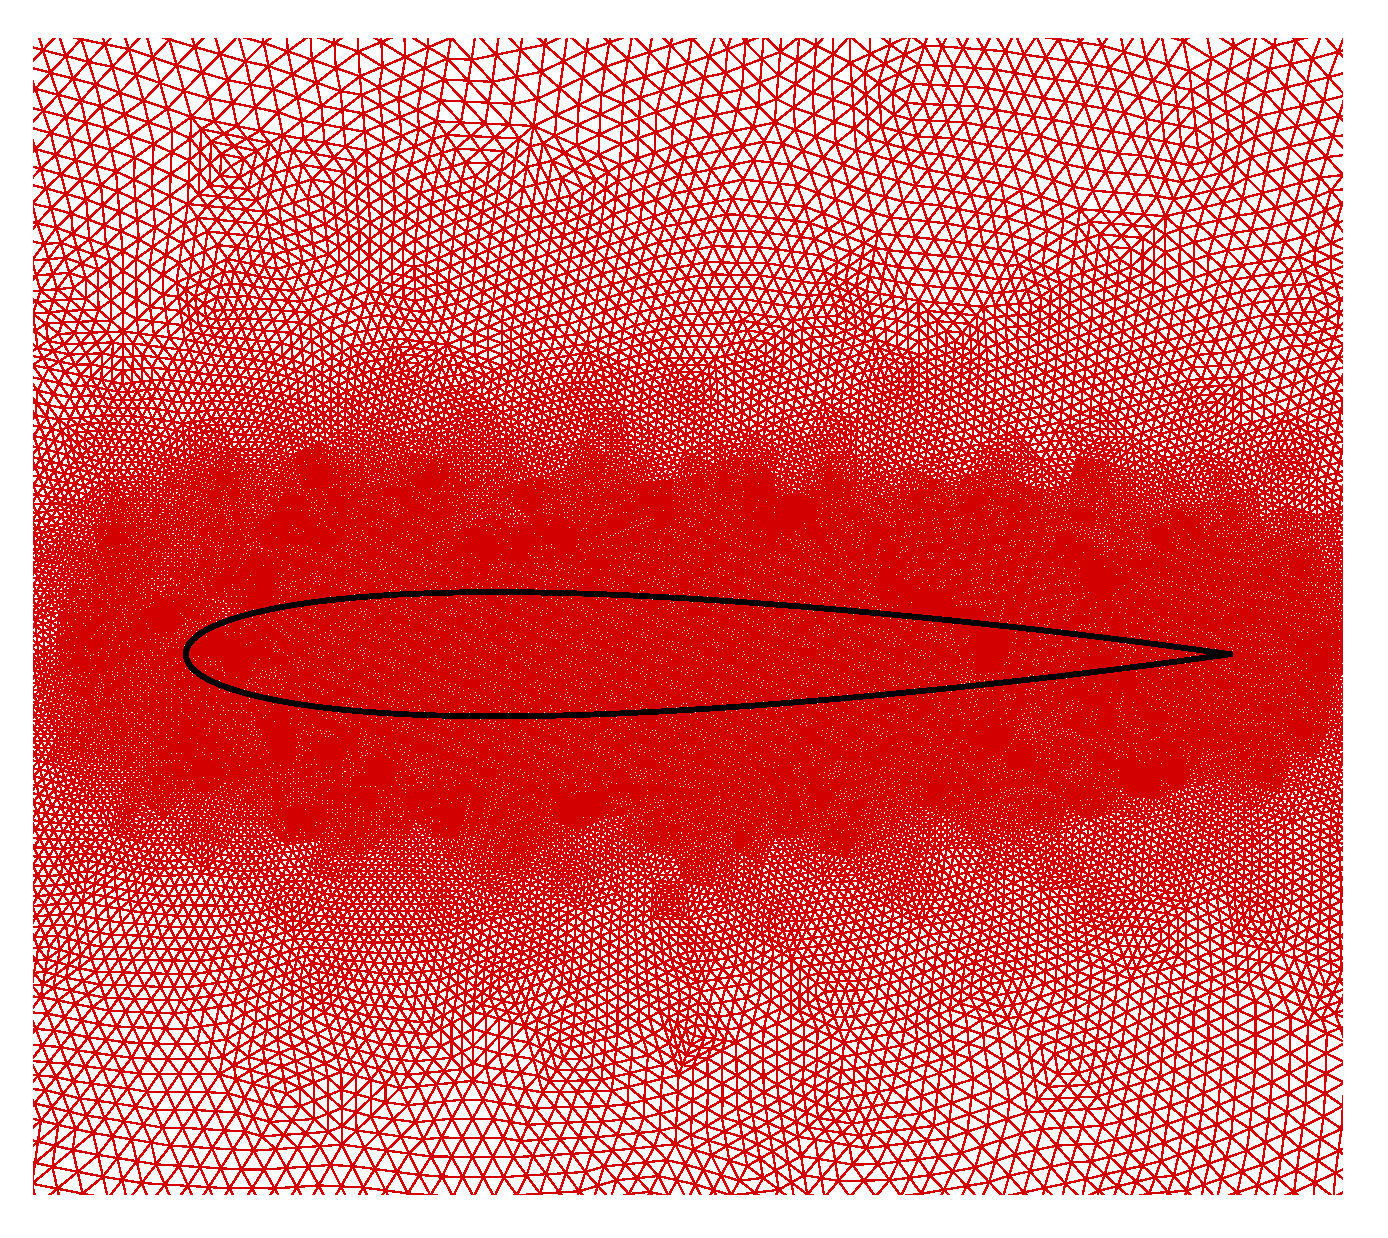
\includegraphics[width=0.42\linewidth]{Fig/mesh_naca_sc}
    \hspace{4mm}
    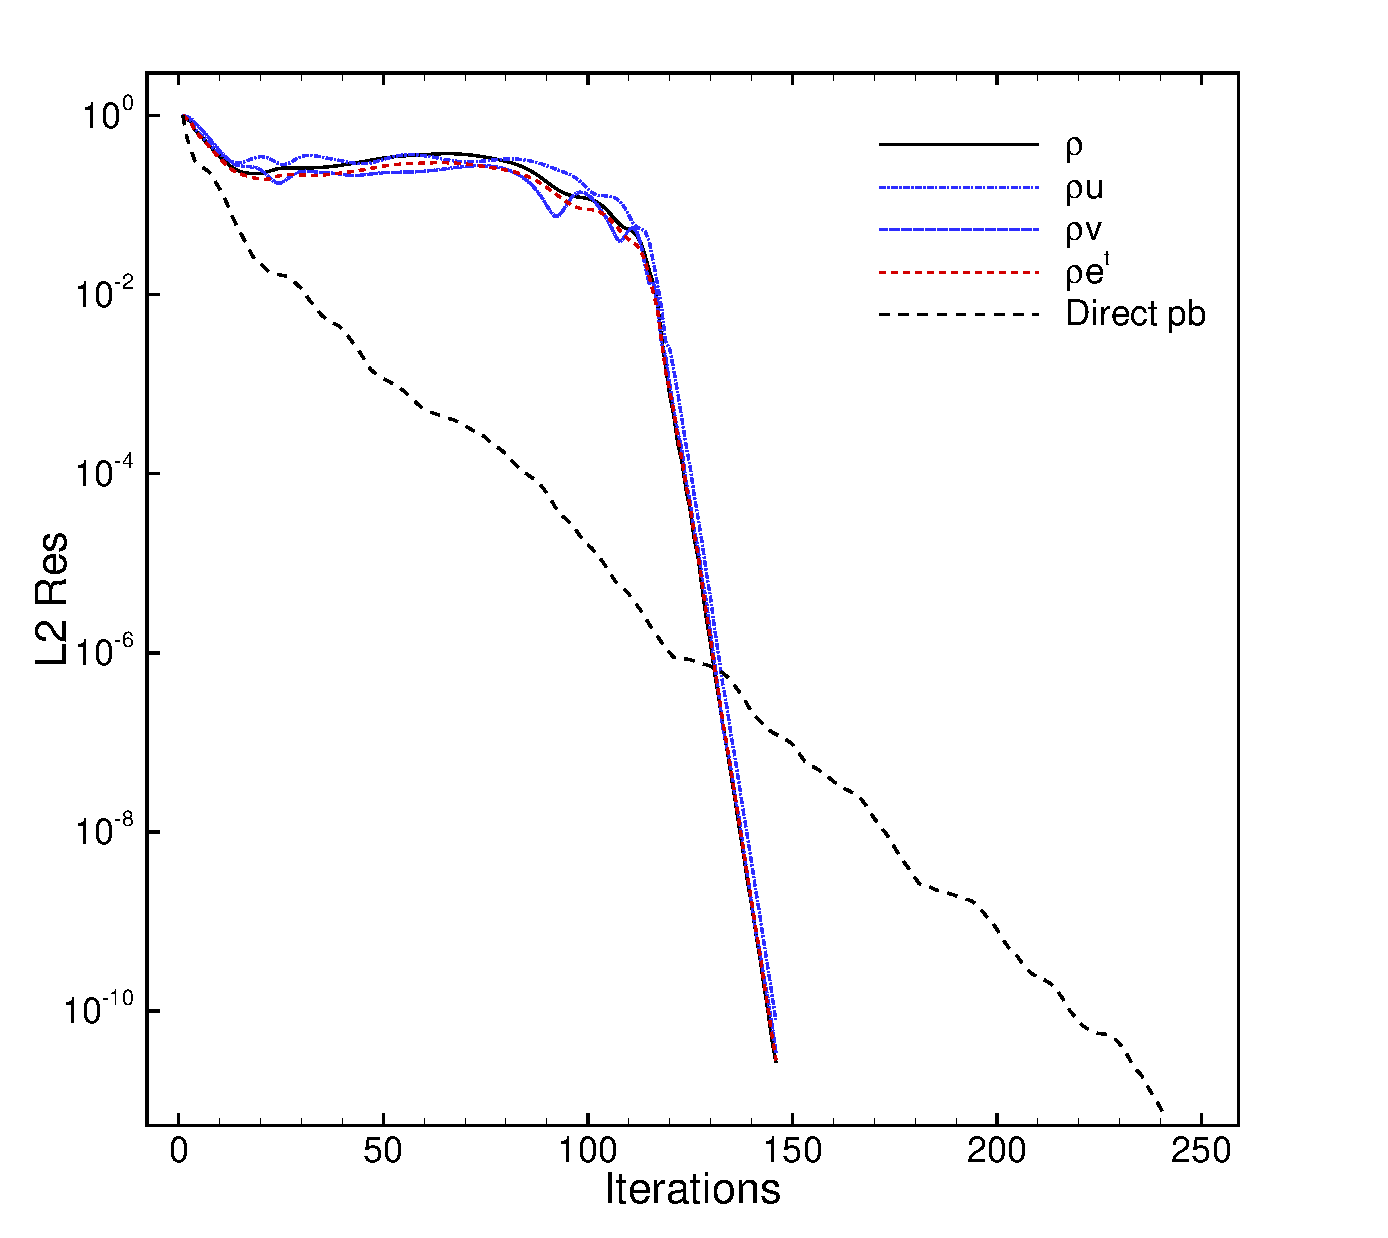
\includegraphics[width=0.43\linewidth]{Fig/res_naca_sc}
  \end{figure}

  \begin{columns}
    \column{0.5\textwidth}
    \begin{itemize}
    \item 3D Grid $\sim 200\,000$ nodes
    \item CFD CPU time $\sim 10$ min
    \item Direct problem CPU time: seconds
    \end{itemize}
    \column{0.5\textwidth}
    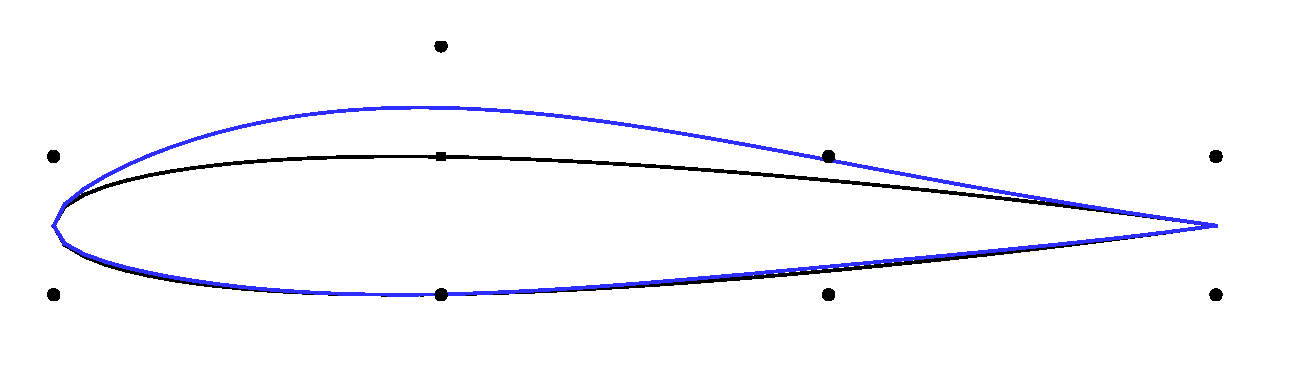
\includegraphics[width=1.0\linewidth]{Fig/ffd}
  \end{columns}
\end{frame}

\begin{frame}
  \frametitle{Verification of the analytical sensitivities}  
  \framesubtitle{NACA-0012, Ma = 0.6, $\alpha=2^\circ$}
  \begin{itemize}
    \item Sensitivity of the lift coefficient 
    \item Relative error between analytical and finite difference derivatives
  \end{itemize}
  \begin{figure}[!ht]
    \centering
    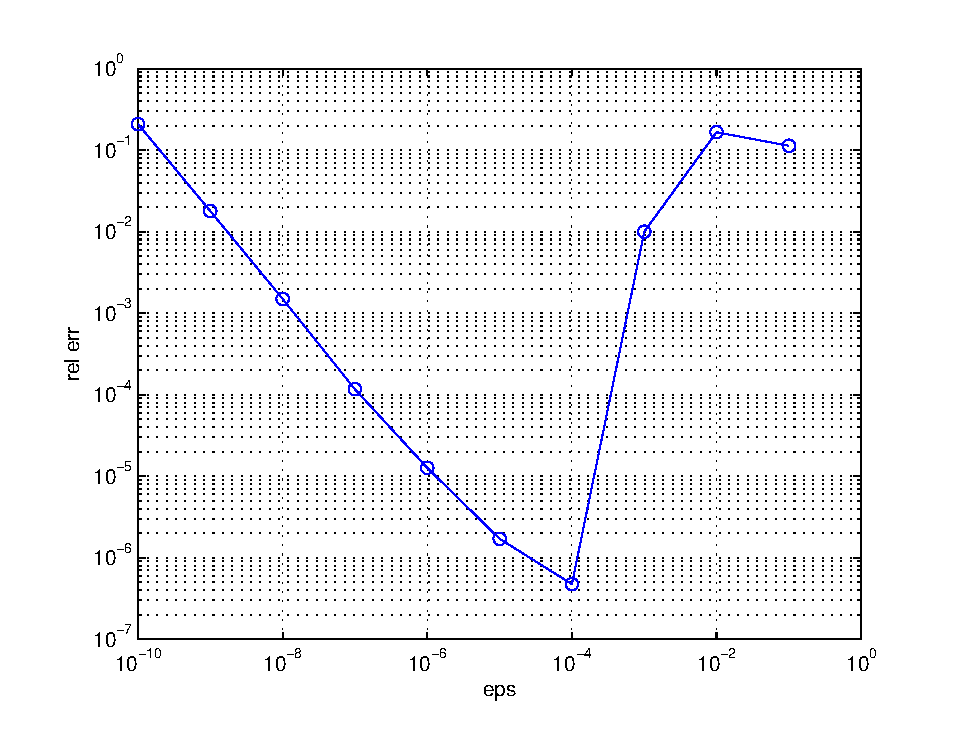
\includegraphics[width=0.6\linewidth]{Fig/err_sc}
  \end{figure}
\end{frame}

%------------------------------------------------------------------------------

\begin{frame}
  \frametitle{Single element airfoil optimization}
  \framesubtitle{NACA-0012, Ma = 0.5, $\alpha=2^\circ$}
  \begin{itemize}
  \item Objective: maximize lift
  \item Cubic design element 
    \begin{itemize}
    \item 8 variables for the displacement of a control node in the vertical direction
    \item 1 displacement constrained to zero to eliminate rigid translations
    \end{itemize}
  \item Second-order spatial discretization
  \item Constraint only on no self-penetration
  \end{itemize}
  \vspace{2mm}
   \begin{figure}
    \centering
    
\includegraphics[width=0.65\textwidth]{Fig/nacadef}
  \end{figure}
\end{frame}

%------------------------------------------------------------------------------

\begin{frame}
  \frametitle{Single element airfoil optimization}
  \framesubtitle{NACA-0012, Ma = 0.5, $\alpha=2^\circ$}
  \begin{itemize}
  \item Optimization converges in $10$ design iterations
  \item Extreme shape deformation handled easily in the IB framework
  \end{itemize}
   \begin{columns}
    \begin{column}{0.5\textwidth}
      \begin{figure}
        \centering
        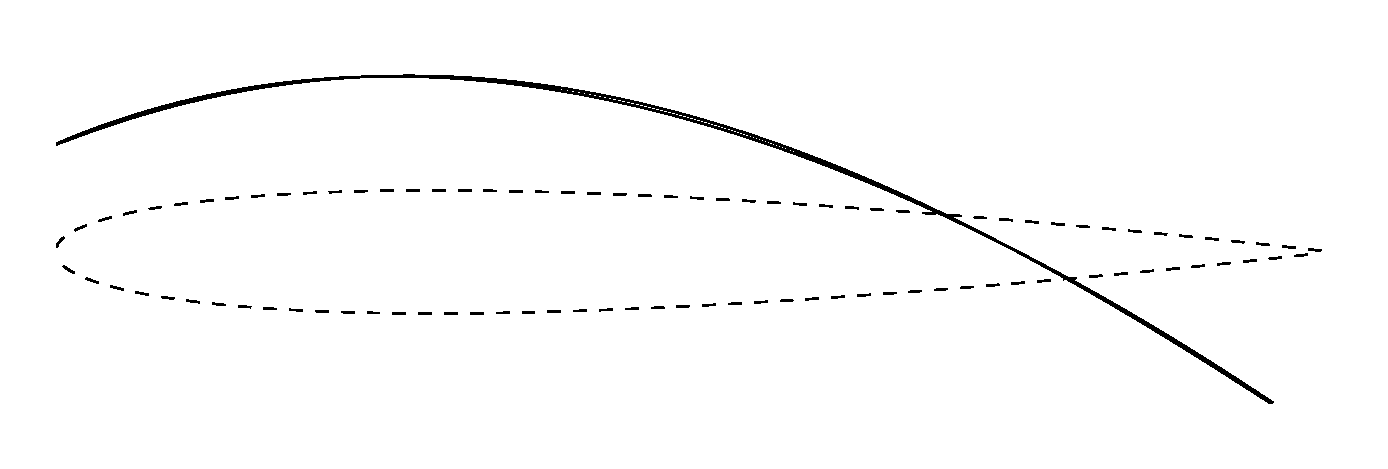
\includegraphics[width=1.0\textwidth]{Fig/naca_def}
      \end{figure}
    \end{column}
    \begin{column}{0.5\textwidth}
      \begin{figure}
        \centering
        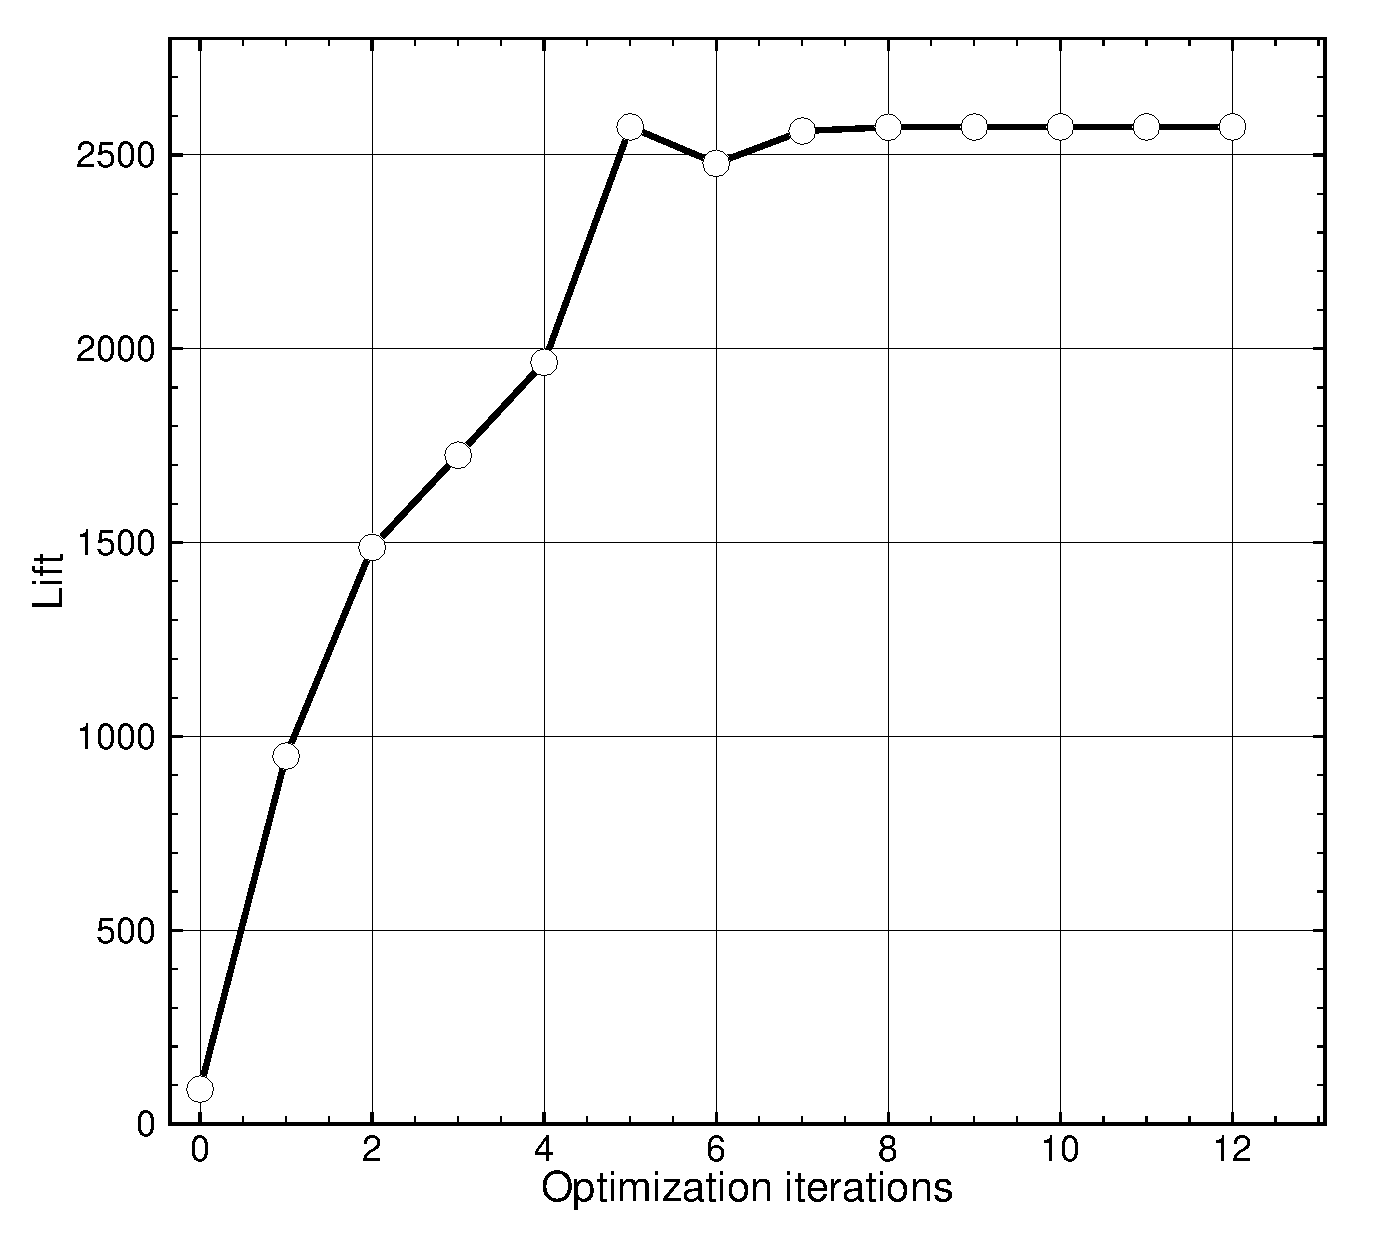
\includegraphics[width=1.0\textwidth]{Fig/L_naca}
      \end{figure}
    \end{column}      
  \end{columns}
\end{frame}

%------------------------------------------------------------------------------

\begin{frame}
  \frametitle{Multi-element airfoil with large kinematics}
  \begin{itemize}
  \item Design of a three-element high-lift configuration
  \item Large number of design variables: geometry perturbation + 
        large displacements and deflections of the slat and flap elements
  \item Maximize the lift by finding the best position of the slat and flap
    elements without introducing any shape modification
  \item Starting from completely closed configuration, let the optimizer find 
    the best relative positions of the airfoil elements
  \end{itemize}
  \begin{figure}
    \centering
    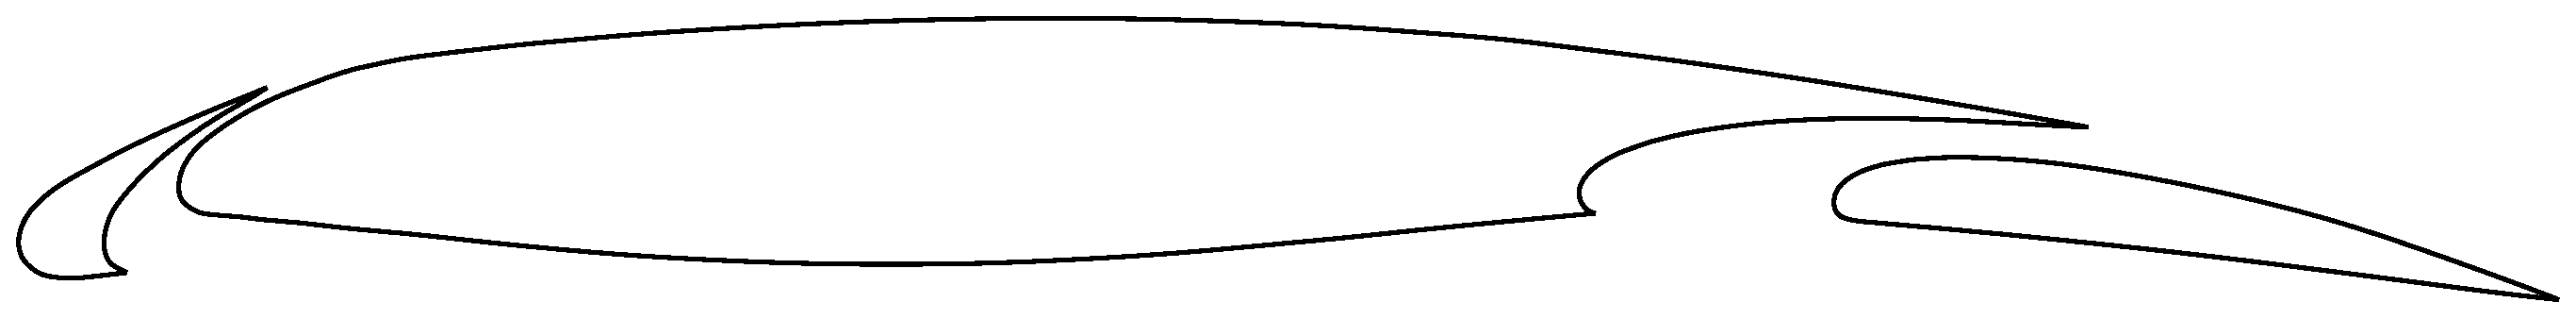
\includegraphics[width=0.8\textwidth]{Fig/L1T2_halfopen}
  \end{figure} 
\end{frame}

%------------------------------------------------------------------------------

\begin{frame}
   \frametitle{Multi-element airfoil with large kinematics}
    \begin{itemize}
    \item 6 design variables: rotation, vertical and horizontal displacements of the
      slat and flap 
    \item Pinball algorithm used to detect contacts between elements and
      avoid interpenetration
    \item Same fluid grid used to perform the previous test case
    \item $Ma = 0.2$ and $\alpha = 10^\circ$
    \item Final value of the lift doubles after 6 optimization iterations
    \end{itemize}
    \begin{figure}
      \centering
      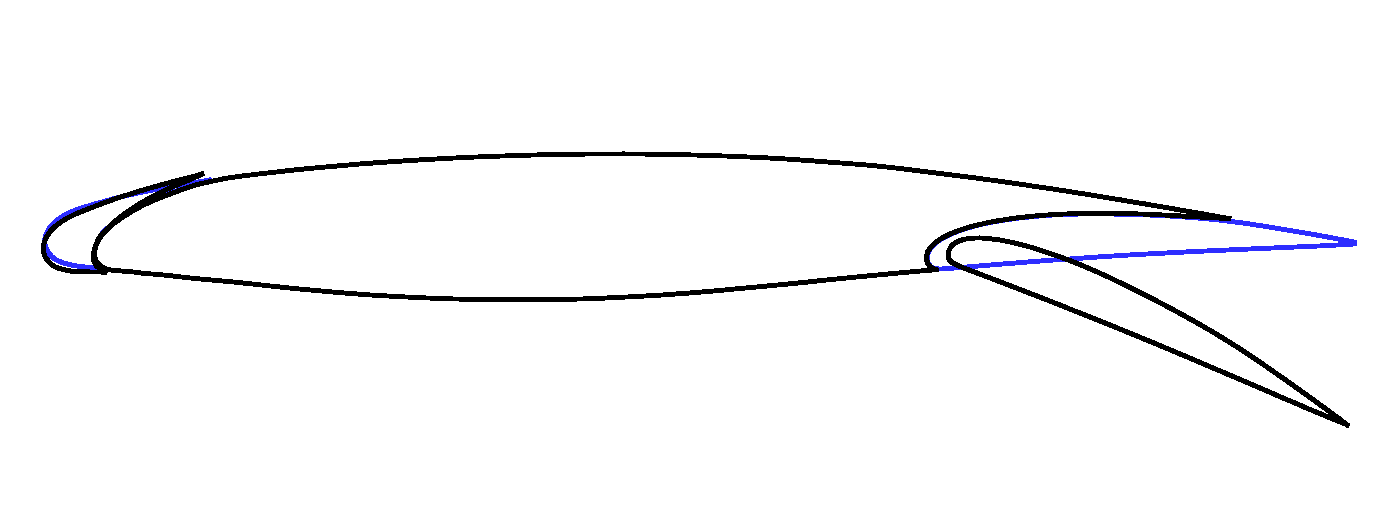
\includegraphics[width=0.8\textwidth]{Fig/L1T2_dep}
     \end{figure}
\end{frame}

\begin{frame}
   \frametitle{Deployment of the multi-element airfoil}
  \begin{center}
    \resizebox{0.9\textwidth}{!}{%
    \animategraphics[autoplay,loop]{10}{Fig/animation}{1}{14}
  }
  \end{center}
\end{frame}

%------------------------------------------------------------------------------

\documentclass[../main.tex]{subfiles}
%\usepackage{algorithm}
%\usepackage{algorithmic}


\everymath{\displaystyle}
\def\arraystretch{2.0}
\begin{document}
\setlength{\delimitershortfall}{0pt}

\chapter{Verification}\label{sec:verification}
\minitoc
%\sectlof
%\sectlot

After chapter~\ref{sec:fluid_mechanics} described the basic equations of fluid mechanics, discretization of this equations with \ac{FV} and \ac{FE} schemes in chapter~\ref{sec:finite_volume_method}, and an introduction to \ac{SA}, the expressions for the actual derivatives have been derived in chapter~\ref{sec:SA}. This has been done for both the body-fitted and the embedded~\ref{sec:embedded_boundary_method} framework of AERO-F.\\
This chapter is denoted to a thorough validation of the obtained derivatives. As described in \ref{sec:SA}, AERO-F handles both sensitivities with respect to far-field variables(e.g. angle of attack) as well as shape sensitivities. Both types require to be handled fundamentally different. While the first type leads to derivatives mainly in the far field boundary conditions, the latter one interferes with the wall treatment. More importantly, as shown in chapters~\ref{sec:fluid_jacobian} and \ref{sec:dresidual_by_absvar}, in the embedded case, doing shape sensitivities leads to additional derivatives with regards to the intersector.\\
For all those reasons, the verification provided in this chapter deals with both $\machnum_{\infty}$-sensitivity as well as shape-sensitivity. More over we will provide plots for both the body-fitted and the embedded case.

\section{Approach}\label{sec:verification_approach}
The question of how to verify the obtained sensitivities is anything but straightforward.\\
The first question is: What can be verified anyway?\\
If we have a look at equation \eqref{eq:full_sa_nostruct}, one can see, that there are two main derivatives: $\pdfrac{\dresidual}{\dfstate}$ and $\pdfrac{\dresidual}{\absvar}$. The derivative with respect to the mesh position $\pdfrac{\dresidual}{\dmpos}$ is not validated here, since it is obtained from SDESIGN and taken for granted.\\
The basic idea that we exploit for verification is to compute a reference solution for the sensitivities by a \ac{FD} of two steady-state simulations. The advantage is, that the sensitivity-module does not have to be used at all to obtain those references, thus it is ensured that potential bugs are not carried over.\\
However, for both of the above quantities, computing a finite difference solution is cumbersome. For the Jacobian $\pdfrac{\dresidual}{\dfstate}$ a simple forward difference would look as follows:
\begin{align}
\pdfrac{\dresidual_i}{\dfstate_j}\bigg\rvert_{\fstate_0}=\frac{\dresidual_i(\dfstate_0+\epsilon\vec{e}_j)-\dresidual_i(\dfstate_0-\epsilon\vec{e}_j)}{2\epsilon}
\end{align}
which would entail an $\order{N}$ number of residual evaluations.\\
As far as $\pdfrac{\dresidual}{\absvar}$ goes, a \ac{FD} verification would be feasible:
\begin{align}
\pdfrac{\dresidual_i}{\machnum_{\infty}}&=\frac{\dresidual(\dfstate_i^{+})-\dresidual(\dfstate_i^{-})}{2\epsilon} \nonumber \\
\dfstate_i^{\pm} &=
\begin{cases}
\dfstate_i\big\rvert_{0}\text{   for internal nodes}\\
\dfstate_i\big\rvert_{\fstate_i(\machnum_i=\machnum_0+\epsilon)}\text{   for boundary nodes}
\end{cases}
\end{align}
which could be done cheaply, and is in fact done in AERO-F if the parameter \texttt{SensitivityAnalysis.SensitivityComputation} is set to \texttt{FiniteDifference}. However, it requires the fluid-state to be updated according to the Mach-number change at the fluid boundary and thus introduces a potential for bugs.\\
Instead, the first quantity to be validated in this thesis is the solution of the linear system described in equation \eqref{eq:full_sa_nostruct}: $\pdfrac{\dfstate}{\absvar}$.\\
this can be done easily by performing a simple \ac{FD} on the solution of two steady-state simulations;
\begin{align}
\tfrac{\dfstate}{\absvar}=\frac{\dfstate(\absvar+\epsilon)-\dfstate(\absvar-\epsilon)}{2 \epsilon}
\end{align}
which involves no extra coding and can be done with a standard steady state solver.
The validation of $\tfrac{\dfstate}{\absvar}$ is provided in figures [\ref{fig:verification_dwdma_ale_Euler},\ref{fig:verification_dwdma_ale_Laminar},\ref{fig:verification_dwdma_ale_RANS}] for the body fitted framework and figures~[\ref{fig:verification_dwdma_emb_Euler},\ref{fig:verification_dwdma_emb_Laminar},\ref{fig:verification_dwdma_emb_RANS}] for the embedded.

Additionally, since the optimization will run on lift and drag, we also validate them with steady state results.
\begin{align}
\tfrac{\optcrit}{\absvar}=\frac{\optcrit(\absvar+\epsilon)-\optcrit(\absvar-\epsilon)}{2 \epsilon}
\end{align}
The validation of integrated forces is provided in figures~[\ref{fig:dLdMa_Euler_ale},\ref{fig:dLdMa_Laminar_ale},\ref{fig:dLdMa_RANS_ale}] for body-fitted computations and in figures~[\ref{fig:dLdMa_Euler_emb},\ref{fig:dLdMa_Laminar_emb},\ref{fig:dLdMa_RANS_emb}] for embedded.



\begin{figure}
\centering
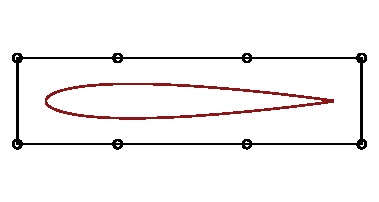
\includegraphics[scale=0.5]{\mainpath/fig/pdf/verificationsetup.pdf}
\caption[Verification setup]{Setup used for the sensitivity verification. A simple NACA0012 profile is considered. The design element concept, as described in section \ref{sec:design_model} is applied. The profile is deformed using a cubic polynomial in x-direction and a linear polynomial in y-direction.}
\label{fig:verification_setup}
\end{figure}


\section{Mach-sensitivity}
For the body-fitted case, the verification of $\tfrac{\dfstate}{\machnum_{\infty}}$ is provided in figure~\ref{fig:verification_dwdma_ale_Euler} for Euler equations, figure~\ref{fig:verification_dwdma_ale_Laminar} for full \ac{NSE} and in figure~\ref{fig:verification_dwdma_ale_RANS} for \ac{NSE} with an additional Spallart-Almares turbulence model.
Additionally, a side by side comparison of the analytic results between all three equation types is also provided in figure~\ref{fig:verification_dwdma_ale_comparison} in order to ensure, that the additional viscous and turbulent terms actually account for a visible difference.\\
For the embedded case, we provide the verification of $\tfrac{\dfstate}{\machnum_{\infty}}$  in figure~\ref{fig:verification_dwdma_emb_Euler} for Euler equation, figure~\ref{fig:verification_dwdma_emb_Laminar} for full \ac{NSE} and in figure~\ref{fig:verification_dwdma_emb_RANS} for \ac{NSE} equations with an additional Spallart-Almares turbulence model.
Again, a side by side comparison of the analytic results between all three equation types is also provided in figure~\ref{fig:verification_dwdma_emb_comparison} in order to ensure that the additional viscous and turbulent terms actually account for a visible difference.


%--------------------------------------------------------------------------------------------
%\section{Body-fitted}
\foreach \vertype in {Euler,Laminar,RANS}{
	%\subsection{Verification $\tfrac{\dfstate}{\machnum_{\infty}}$ for \vertype equations and a body-fitted framework}
	\begin{figure}[t!]
	    \centering
	    \textbf{Verification $\tfrac{\dfstate}{\machnum_{\infty}}$ for {\vertype} equations and a body-fitted framework}\par\medskip    
	    \foreach \n in {1,2,3,5}{
	      \foreach \type in {FD,ana}{
			    \begin{subfigure}[t]{0.4\textwidth}
			        \centering
			        \setlength{\fboxsep}{\valfboxsep}%\valfboxsep=0pt
              \setlength{\fboxrule}{\valfboxrule}%\valfboxrule=1pt
			        \fbox{\includegraphics[width=\linewidth]{\mainpath/fig/studies/StateVector_verification/machsens/ALE/\vertype_component\n_\type}}
			        \caption{$\linepdfrac{\d{w}_\n^{\type}}{\machnum_{\infty}}$}
			    \end{subfigure}%
			    ~ 
	      }~
	      \begin{subfigure}[t]{0.1\textwidth}
	        
\includegraphics[width=0.22\linewidth]{\mainpath/fig/studies/StateVector_verification/colorbar_empty}
	      \end{subfigure}
	      
	    }
	    \caption[Verification $\tfrac{\dfstate}{\machnum_{\infty}}$ {\vertype} equations body-fitted]{Verification of $\tfrac{\dfstate}{\machnum_{\infty}}$ for {\vertype} equations in the body-fitted framework. The \ac{FD} reference solution as described in chapter~\ref{sec:verification_approach} is provided in the left column, the newly implemented analytic derivatives are visualized in the right column. \ac{FD} and analytic solution are plotted using the same color-scheme.}
	    \label{fig:verification_dwdma_ale_\vertype}
	    
	    
	\end{figure}
}

%--------------------------------------------------------------------------------------------
%\section{Embedded}
\foreach \vertype in {Euler,Laminar,RANS}{
	%\subsection{Verification of the \vertype derivatives}
	\begin{figure}[t!]
	    \centering
	    \textbf{Verification of $\tfrac{\dfstate}{\machnum_{\infty}}$ for {\vertype} equations and a embedded framework}\par\medskip    
	    \foreach \n in {1,2,3,5}{
	      \foreach \type in {FD,ana}{
			    \begin{subfigure}[t]{0.4\textwidth}
			        \centering
			        \setlength{\fboxsep}{\valfboxsep}%\valfboxsep=0pt
              \setlength{\fboxrule}{\valfboxrule}%\valfboxrule=1pt
			        \fbox{\includegraphics[width=\linewidth]{\mainpath/fig/studies/StateVector_verification/machsens/Emb/\vertype_component\n_\type}}
			        \caption{$\linepdfrac{\d{w}_\n^{\type}}{\machnum_{\infty}}$}
			    \end{subfigure}%
			    ~ 
	      }~
	      \begin{subfigure}[t]{0.1\textwidth}
	        
\includegraphics[width=0.22\linewidth]{\mainpath/fig/studies/StateVector_verification/colorbar_empty}
	      \end{subfigure}
	      
	    }
	    \caption[Verification of $\tfrac{\dfstate}{\machnum_{\infty}}$ for {\vertype} equations, embedded]{Verification of $\tfrac{\dfstate}{\machnum_{\infty}}$ for {\vertype} equations in the embedded framework. The \ac{FD} reference solution as described in chapter~\ref{sec:verification_approach} is provided in the left column, the newly implemented analytic derivatives are visualized in the right column. \ac{FD} and analytic solution are plotted using the same color-scheme.}
	    \label{fig:verification_dwdma_emb_\vertype}
	    
	\end{figure}
}





%--------------------------------------------------------------------------------------------
%\subsection{Comparison}

\begin{figure}[t!]
    \centering
    \textbf{Comparison of $\tfrac{\dfstate}{\machnum_{\infty}}$ in the body-fitted framework for all 3 equation types}\par\medskip    
    \foreach \n in {1,2,3,5}{
      \foreach \simtype in {Euler,Laminar,RANS}{
		    \begin{subfigure}[t]{0.3\textwidth}
		        \centering
			        \setlength{\fboxsep}{\valfboxsep}%\valfboxsep=0pt
              \setlength{\fboxrule}{\valfboxrule}%\valfboxrule=1pt
		        \fbox{\includegraphics[width=\linewidth]{\mainpath/fig/studies/StateVector_verification/machsens/ALE/comparison_\simtype_component\n_ana}}
		        \caption{$\linepdfrac{\d{w_\n^{\simtype}}}{\machnum_{\infty}}$}
		    \end{subfigure}%
		    ~ 
      }~
	    \begin{subfigure}[t]{0.1\textwidth}
	      
\includegraphics[width=0.19\linewidth]{\mainpath/fig/studies/StateVector_verification/colorbar_empty}
	    \end{subfigure}
      
    }
    \caption[Comparison of analytic $\tfrac{\dfstate}{\machnum_{\infty}}$ for all equation types body-fitted]{Comparison of analytic $\tfrac{\dfstate}{\machnum_{\infty}}$ for Euler equations(left column), laminar \ac{NSE} equations (center column) and \ac{NSE} equations with turbulence models (right column) in the body-fitted framework.}
    \label{fig:verification_dwdma_ale_comparison}
\end{figure}


\begin{figure}[t!]
    \centering
    \textbf{Comparison of $\tfrac{\dfstate}{\machnum_{\infty}}$ in the embedded framework for all 3 equation types}\par\medskip    
    \foreach \n in {1,2,3,5}{
      \foreach \simtype in {Euler,Laminar,RANS}{
		    \begin{subfigure}[t]{0.3\textwidth}
		        \centering
			        \setlength{\fboxsep}{\valfboxsep}%\valfboxsep=0pt
              \setlength{\fboxrule}{\valfboxrule}%\valfboxrule=1pt
		        \fbox{\includegraphics[width=\linewidth]{\mainpath/fig/studies/StateVector_verification/machsens/Emb/comparison_\simtype_component\n_ana}}
		        \caption{$\linepdfrac{\d{w_\n^{\simtype}}}{\machnum_{\infty}}$}
		    \end{subfigure}%
		    ~ 
      }~
	    \begin{subfigure}[t]{0.1\textwidth}
	      
\includegraphics[width=0.19\linewidth]{\mainpath/fig/studies/StateVector_verification/colorbar_empty}
	    \end{subfigure}
      
    }
    \caption[Comparison of analytic $\tfrac{\dfstate}{\machnum_{\infty}}$ for all equation types embedded]{Comparison of analytic $\tfrac{\dfstate}{\machnum_{\infty}}$ for Euler equations(left column), laminar \ac{NSE} equations (center column) and \ac{NSE} equations with turbulence models (right column) in the embedded framework.}
    \label{fig:verification_dwdma_emb_comparison}
\end{figure}



\FloatBarrier

%--------------------------------------------------------------------------------------------
%--------------------------------------------------------------------------------------------


\section{Shape-sensitivity}
The verification of $\tfrac{\dfstate}{\absvar}$ for body-fitted simulations is provided in figure~\ref{fig:verification_dwds_ale_Euler} for Euler equation, figure~\ref{fig:verification_dwds_ale_Laminar} for full \ac{NSE} and in figure~\ref{fig:verification_dwds_ale_RANS} for \ac{NSE} with an additional Spallart-Almares turbulence model.
Additionally, a side by side comparison of the analytic results between all three equation types is also provided in figure~\ref{fig:verification_dwds_ale_comparison} in order to ensure that the additional viscous and turbulent terms actually account for a visible difference.
\\
For the embedded case, we provide the verification of $\tfrac{\dfstate}{\absvar}$  in figure~\ref{fig:verification_dwds_emb_Euler} for Euler equation, figure~\ref{fig:verification_dwds_emb_Laminar} for full \ac{NSE} and in figure~\ref{fig:verification_dwds_emb_RANS} for \ac{NSE} with an additional Spallart-Almares turbulence model.
Again, a side by side comparison of the analytic results between all three equation types is also provided in figure~\ref{fig:verification_dwds_emb_comparison} in order to ensure that the additional viscous and turbulent terms actually account for a visible difference.
%--------------------------------------------------------------------------------------------
%\section{Body-fitted}
\foreach \vertype in {Euler,Laminar,RANS}{
	%\subsection{Verification of the \vertype derivatives}
	\begin{figure}[t!]
	    \centering
	    \textbf{Verification $\tfrac{\dfstate}{\absvar}$ for {\vertype} equations and a body-fitted framework}\par\medskip    
	    \foreach \n in {1,2,3,5}{
	      \foreach \type in {FD,ana}{
			    \begin{subfigure}[t]{0.4\textwidth}
			        \centering
			        \setlength{\fboxsep}{\valfboxsep}%\valfboxsep=0pt
              \setlength{\fboxrule}{\valfboxrule}%\valfboxrule=1pt
			        \fbox{\includegraphics[width=\linewidth]{\mainpath/fig/studies/StateVector_verification/shapesens/ALE/\vertype_component\n_\type}}
			        \caption{$\linepdfrac{\d{w}_\n^{\type}}{\absvar}$}
			    \end{subfigure}%
			    ~ 
	      }~
	      \begin{subfigure}[t]{0.1\textwidth}
	        
\includegraphics[width=0.22\linewidth]{\mainpath/fig/studies/StateVector_verification/colorbar_empty}
	      \end{subfigure}
	      
	    }
	    \caption[Verification of $\tfrac{\dfstate}{\absvar}$ {\vertype} for equations, body-fitted]{Verification of $\tfrac{\dfstate}{\absvar}$ for {\vertype} equations in the body-fitted framework.
	    The \ac{FD} reference solution as described in chapter~\ref{sec:verification_approach} is provided in the left column, the newly implemented analytic derivatives are visualized in the right column. \ac{FD} and analytic solution are plotted using the same color-scheme.}
	    \label{fig:verification_dwds_ale_\vertype}
	    
	\end{figure}
}

%--------------------------------------------------------------------------------------------
%\section{Embededd}

\foreach \vertype in {Euler,Laminar,RANS}{
	%\subsection{Verification of the \vertype derivatives}
	\begin{figure}[t!]
	    \centering
	    \textbf{Verification $\tfrac{\dfstate}{\absvar}$ for {\vertype} equations and a embedded framework}\par\medskip    
	    \foreach \n in {1,2,3,5}{
	      \foreach \type in {FD,ana}{
			    \begin{subfigure}[t]{0.4\textwidth}
			        \centering
			        \setlength{\fboxsep}{\valfboxsep}%\valfboxsep=0pt
              \setlength{\fboxrule}{\valfboxrule}%\valfboxrule=1pt
			        \fbox{\includegraphics[width=\linewidth]{\mainpath/fig/studies/StateVector_verification/shapesens/Emb/\vertype_component\n_\type}}
			        \caption{$\linepdfrac{\d{w}_\n^{\type}}{\absvar}$}
			    \end{subfigure}%
			    ~ 
	      }~
	      \begin{subfigure}[t]{0.1\textwidth}
	        
\includegraphics[width=0.22\linewidth]{\mainpath/fig/studies/StateVector_verification/colorbar_empty}
	      \end{subfigure}
	      
	    }
	    \caption[Verification $\tfrac{\dfstate}{\absvar}$ {\vertype} equations embedded]{Verification of $\tfrac{\dfstate}{\absvar}$ for {\vertype} equations in the embedded framework.
	    The \ac{FD} reference solution as described in chapter~\ref{sec:verification_approach} is provided in the left column, the newly implemented analytic derivatives are visualized in the right column. \ac{FD} and analytic solution are plotted using the same color-scheme.}
	    \label{fig:verification_dwds_emb_\vertype}
	    
	\end{figure}
}


%--------------------------------------------------------------------------------------------
%\subsection{Comparison}

\begin{figure}[t!]
    \centering
    \textbf{Comparison of $\tfrac{\dfstate}{\absvar}$ in the body-fitted framework for all 3 equation types}\par\medskip    
    \foreach \n in {1,2,3,5}{
      \foreach \simtype in {Euler,Laminar,RANS}{
		    \begin{subfigure}[t]{0.3\textwidth}
		        \centering
			        \setlength{\fboxsep}{\valfboxsep}%\valfboxsep=0pt
              \setlength{\fboxrule}{\valfboxrule}%\valfboxrule=1pt
		        \fbox{\includegraphics[width=\linewidth]{\mainpath/fig/studies/StateVector_verification/shapesens/ALE/\simtype_component\n_ana}}
		        \caption{$\linepdfrac{\d{w_\n^{\simtype}}}{\absvar}$}
		    \end{subfigure}%
		    ~ 
      }~
	    \begin{subfigure}[t]{0.1\textwidth}
	      
\includegraphics[width=0.19\linewidth]{\mainpath/fig/studies/StateVector_verification/colorbar_empty}
	    \end{subfigure}
      
    }
    \caption[Comparison of analytic $\tfrac{\dfstate}{\machnum_{\infty}}$ for all equation types, body-fitted]{Comparison of analytic $\tfrac{\dfstate}{\machnum_{\infty}}$ for Euler equations(left column), laminar \ac{NSE} equations (center column) and \ac{NSE} equations with turbulence models (right column) in the body-fitted framework.}
    \label{fig:verification_dwds_ale_comparison}
\end{figure}

\begin{figure}[t!]
    \centering
    \textbf{Comparison of $\tfrac{\dfstate}{\absvar}$ in the embedded framework for all 3 equation types}\par\medskip    
    \foreach \n in {1,2,3,5}{
      \foreach \simtype in {Euler,Laminar,RANS}{
		    \begin{subfigure}[t]{0.3\textwidth}
		        \centering
			        \setlength{\fboxsep}{\valfboxsep}%\valfboxsep=0pt
              \setlength{\fboxrule}{\valfboxrule}%\valfboxrule=1pt
		        \fbox{\includegraphics[width=\linewidth]{\mainpath/fig/studies/StateVector_verification/shapesens/Emb/\simtype_component\n_ana}}
		        \caption{$\linepdfrac{\d{w_\n^{\simtype}}}{\absvar}$}
		    \end{subfigure}%
		    ~ 
      }~
	    \begin{subfigure}[t]{0.1\textwidth}
	      
\includegraphics[width=0.19\linewidth]{\mainpath/fig/studies/StateVector_verification/colorbar_empty}
	    \end{subfigure}
      
    }
    \caption[Comparison of analytic $\tfrac{\dfstate}{\machnum_{\infty}}$ for all equation types, embedded]{Comparison of analytic $\tfrac{\dfstate}{\machnum_{\infty}}$ for Euler equations(left column), laminar \ac{NSE} equations (center column) and \ac{NSE} equations with turbulence models (right column) in the embedded framework.}
    \label{fig:verification_dwds_emb_comparison}
\end{figure}






\end{document}






\section{Examples}

\begin{frame}
\frametitle{Multi-element airfoil with large kinematics}
\framesubtitle{Prime example for embedded framework}
\begin{figure}
\setlength{\fboxsep}{\valfboxsep}%\valfboxsep=0pt
\setlength{\fboxrule}{\valfboxrule}%\valfboxrule=1pt      
\foreach \n in {1,2,3,5,6,7,8,9,10,11,12,13,14}{
\centering
\only<\n>{\fbox{\includegraphics[width=0.90\paperwidth]{/home/lukas/Desktop/project/independence/project/thesis/fig/png/multielem_euler/animation\n.jpg}}}
\only<\n>{\caption{Optimization iteration \n}}
%\only<2>{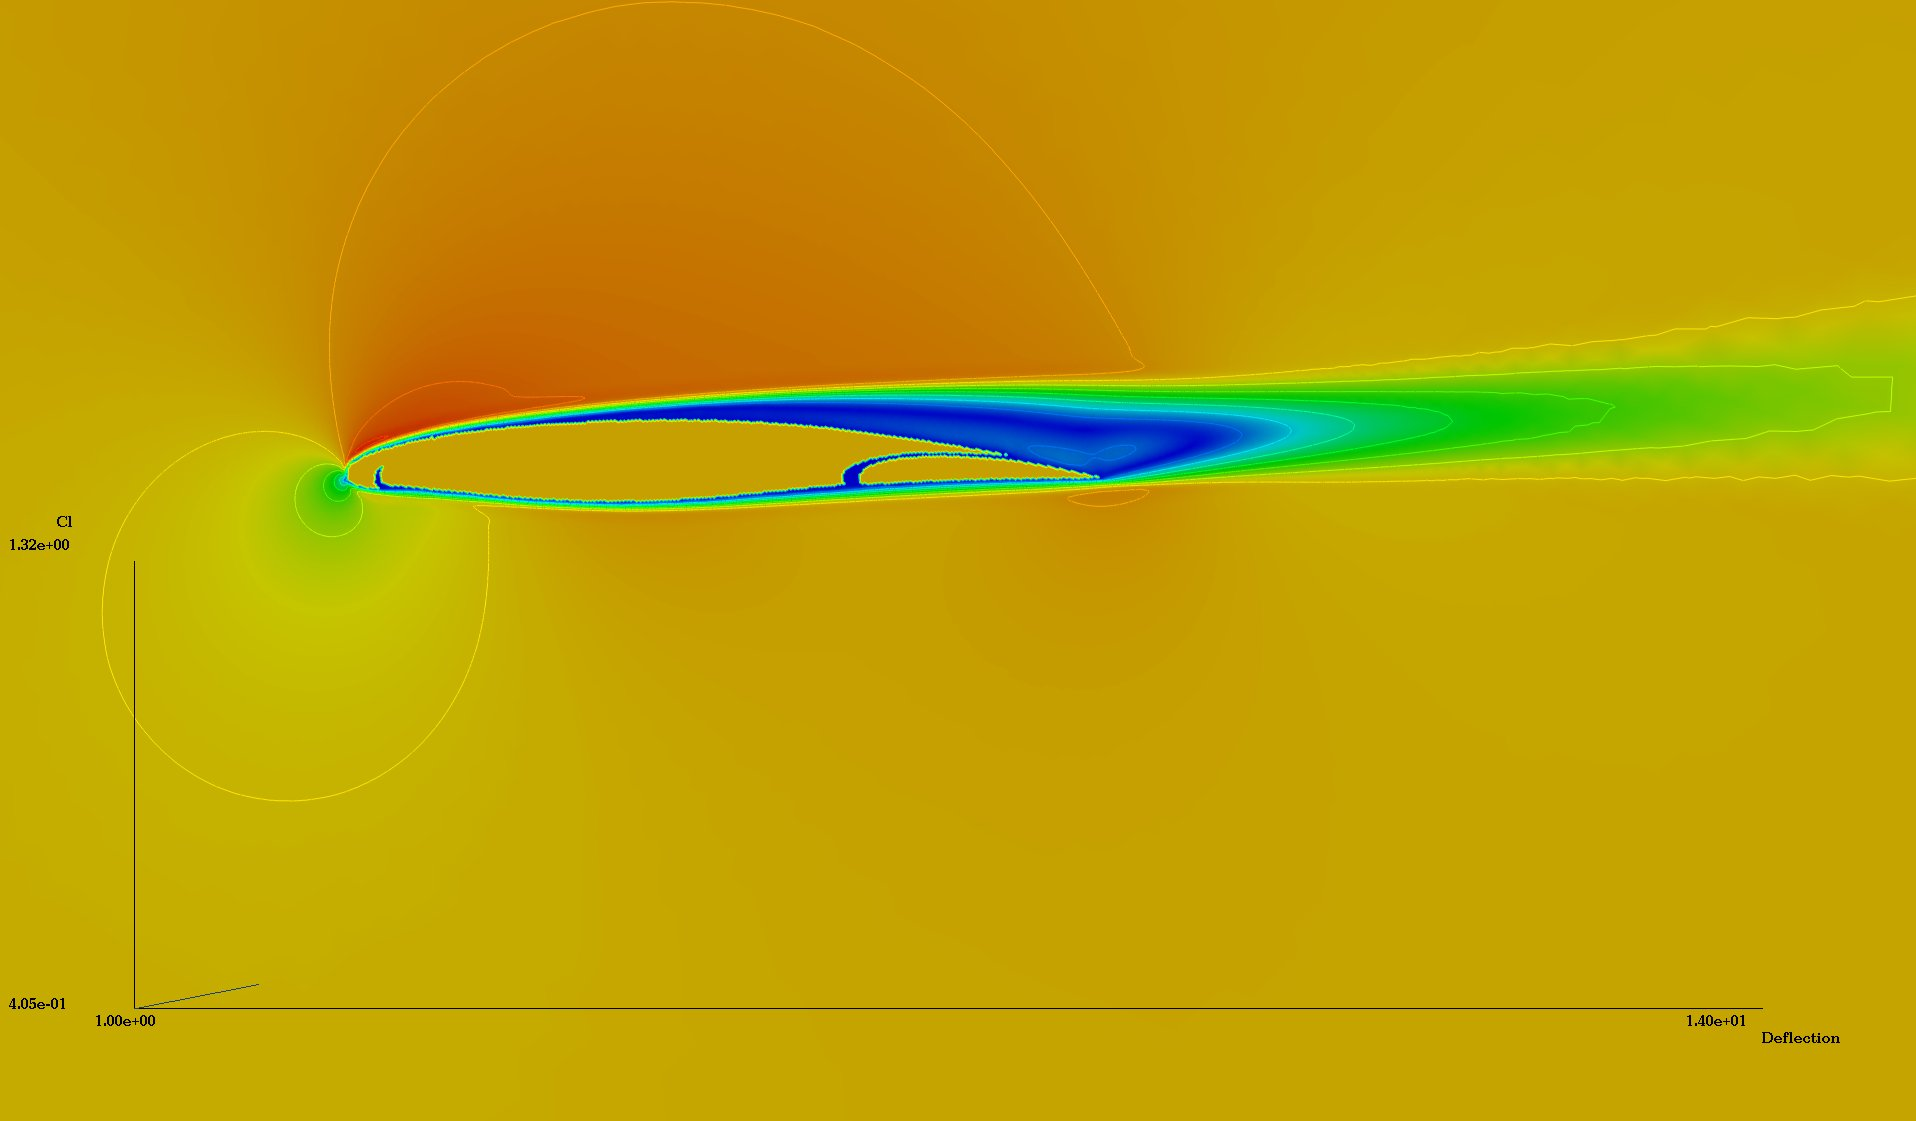
\includegraphics[width=10cm]{/home/lukas/Desktop/project/independence/project/thesis/fig/png/multielem_euler/animation2.jpg}}
}
\end{figure}
\end{frame}

%------------------------------------------------------------------------------

\begin{frame}
\frametitle{Multi-element airfoil with large kinematics}
\framesubtitle{Prime example for embedded framework}
\begin{figure}
\fbox{\includegraphics[width=0.90\paperwidth]{/home/lukas/Desktop/project/independence/Talk.d/Fig/animation_final.jpg}}
\end{figure}
\begin{itemize}
\item{$\machnum=0.2$ and $\alpha=10^{\circ}$}
\item{Starting from closed configuration; let optimizer find the best relative positions of the airfoil elements}
\item{6 design variables: rotation, vertical and horizontal displacement of the elements}
\item{Final value of the lift doubles after 6 optimization iterations}
\end{itemize}
\end{frame}
%\documentclass[../main.tex]{subfiles}
%\usepackage{algorithm}
%\usepackage{algorithmic}


\everymath{\displaystyle}
\def\arraystretch{2.0}
\def\naca0012path{/home/lukas/Desktop/project/independence/project/simulations/naca0012}
\begin{document}
\setlength{\delimitershortfall}{0pt}

\FloatBarrier 
\chapter{Conclusions}\label{sec:conclusions}
%\addcontentsline{lof}{chapter}{Conclusions}
\minitoc
%\sectlof
%\sectlot

\section{Summary}\label{sec:summary}
This thesis began with a short motivation on why analytic sensitivity analysis is desirable and what applications in the context of optimization look like. We then provided a quick overview on the basic equations of fluid mechanics in section~\ref{sec:fluid_mechanics}. Particularly, we put emphasis on important issues for the subsequent chapters, like Eulerian and Lagrangian view or turbulence models.
The \acf{FV} method has then been introduced in section~\ref{sec:finite_volume_method} as a mean of solving those equations numerically. This chapter followed closely the \av{FV} approach used in AERO-F\cite{Aerof}, the flow solver at the \acf{FRG} at Stanford University. This code has a comprehensive \acf{IBM} framework: \acf{FIVER}\cite{Main2014}. While not restricted to it, this thesis largely dealt with immersed boundaries, the body-fitted case being regarded as a subset.\\
The thesis then shifted towards motivating \acf{SA} by introducing the basics of aerodynamic shape optimization in section~\ref{sec:optimization}, more precisely, gradient-based optimization.
The derivation of these gradients in an analytic manner has been the main focus of the thesis and was introduced in section~\ref{sec:SA} for fluid equations, and section~\ref{sec:aeroelastic_sa} for coupled fluid-structure interaction problems.\\
The theory covered both, the direct and the adjoint method, the implementation was focused on implementing the direct method first.\\
Details on how to evaluate a number of particularly interesting derivatives have been provided in section~\ref{sec:dresidual_derivative}.\\
The implemented analytic derivatives have undergone thorough verification in section~\ref{sec:verification} before they have been applied to simple demonstrative examples in section~\ref{sec:examples}.

\section{Outlook}\label{sec:outlook}
We have successfully demonstrated the feasibility of  analytic sensitivity analysis with an \acf{IBM} and fully viscous and turbulent flows.\\
In combination with the \acf{FIVER}, this offers a very promising framework for aerodynamic and aeroelastic shape optimization. By utilizing the \ac{IBM} we have been able to optimize complex and greatly changing geometries, that would not have been possible in a body-fitted framework, or would at least have required some sort of re-meshing algorithm. The examples delivered promising results for both inviscid and viscous flows.\\
So far, all examples and verifications have been run on first-order simulations. Future effort should therefore focus on the validation of the implemented framework on higher order schemes.\\
Overall, the developed framework represents a powerful and comprehensive tool for gradient-based aerodynamic shape optimization. The \ac{IBM} framework offers unprecedented flexibility with regards to the geometry while greatly improving both the computational efficiency as well as numerical stability compared to \ac{FD}-based gradients.



\end{document}
% -----------------------------------------------------------------------------


% APPENDIX --------------------------------------------------------------------
%\appendix
%\backupbegin
%\documentclass[../main.tex]{subfiles}
%\usepackage{algorithm}
%\usepackage{algorithmic}

\everymath{\displaystyle}
\def\arraystretch{2.0}
\begin{document}
\setlength{\delimitershortfall}{0pt}

\chapter{Appendix}

\subsection{Diffusive tensor $\difftensor$}

The diffusive tensor $\difftensor$ is a fourth order tensor that can be interpreted as a matrix of matrices.
For ideal gas, it reads,

\def\koo{-\frac{4 \fluidvelx}{3} }
\def\ktt{ \frac{4}{3} }
\def\keo{ \fluidvely }
\def\kee{ 1 }
\def\kao{ \fluidvelz }
\def\kaa{ 1 }
\def\kto{ -\frac{4\fluidvelx}{3} }

\def\kso{ -\Big((1-\frac{\gamma}{Pr})\norm{\fluidvel}^2+\frac{\fluidvelx^2}{3}+\frac{\gamma E}{Pr} \Big) }
\def\kst{ \fluidvelx(\frac{4}{3}-\frac{\gamma}{Pr}) }
\def\kse{ \fluidvely(1-\frac{\gamma}{Pr}) }
\def\ksa{ \fluidvelz(1-\frac{\gamma}{Pr}) }
\def\kss{ \frac{\gamma}{Pr} }
\begin{align}\nonumber
\difftensor_{11}=\frac{\mu}{\dens}
\begin{bmatrix}
  0     &    0     &    0     &    0     &    0     \\
  \kto  &    \ktt  &    0     &    0     &    0     \\
  \keo  &    0     &    \kee  &    0     &    0     \\
  \kao  &    0     &    0     &    \kaa  &    0     \\
  \kso  &    \kst  &    \kse  &    \ksa  &    \kss  \\
\end{bmatrix}
\end{align}





\begin{minipage}{0.5\textwidth}
\def\kto{ \frac{2\fluidvely}{3} }
\def\keo{ -\fluidvelx }
\def\kso{ -\frac{\fluidvelx\fluidvely}{3} }
\def\ket{ 1 }
\def\kst{ \fluidvely }
\def\kte{ -\frac{2}{3} }
\def\kse{ -\frac{2\fluidvelx}{3} }
\begin{align}\nonumber
\difftensor_{12}=\frac{\mu}{\dens}
\begin{bmatrix}
  0     &    0     &    0     &    0     &    0     \\
  \kto  &    0     &    \kte  &    0     &    0     \\
  \keo  &    \ket  &    0     &    0     &    0     \\
  0     &    0     &    0     &    0     &    0     \\
  \kso  &    \kst  &    \kse  &    0     &    0     \\
\end{bmatrix}
\end{align}
\end{minipage}
\begin{minipage}{0.5\textwidth}
\def\kto{ \frac{2\fluidvelz}{3} }
\def\kao{ -\fluidvelx }
\def\kso{ -\frac{\fluidvelx\fluidvelz}{3} }
\def\kao{ -\fluidvelx }
\def\kat{ 1 }
\def\kst{ \fluidvelz }
\def\kta{ -\frac{2}{3} }
\def\ksa{ -\frac{2\fluidvelx}{3} }
\begin{align}\nonumber
\difftensor_{13}=\frac{\mu}{\dens}
\begin{bmatrix}
% o          t          e          a          s
  0     &    0     &    0     &    0     &    0     \\ %o
  \kto  &    0     &    0     &    \kta  &    0     \\ %t
  0     &    0     &    0     &    0     &    0     \\ %e
  \kao  &    \kat  &    0     &    0     &    0     \\ %a
  \kso  &    \kst  &    0     &    \ksa  &    0     \\ %s
\end{bmatrix}
\end{align}

\end{minipage}










\def\kto{ -\fluidvelx }
\def\keo{ -\frac{4\fluidvely}{3} }
\def\kao{ -\fluidvelz }
\def\kso{ -\Big((1-\frac{\gamma}{Pr})\norm{\fluidvel}^2+\frac{\fluidvely^2}{3}+\frac{\gamma E}{Pr} \Big)  }
\def\ktt{ 1 }
\def\kst{ \fluidvelx(1-\frac{\gamma}{Pr}) }
\def\kee{ \frac{4}{3} }
\def\kse{ \fluidvely(\frac{4}{3}-\frac{\gamma}{Pr}) }
\def\kaa{ 1 }
\def\ksa{ \fluidvelz(1-\frac{\gamma}{Pr}) }
\def\kss{ \frac{\gamma}{Pr} }
\begin{align}\nonumber
\difftensor_{22}=\frac{\mu}{\dens}
\begin{bmatrix}
% o          t          e          a          s
  0     &    0     &    0     &    0     &    0     \\ %o
  \kto  &    \ktt  &    0     &    0     &    0     \\ %t
  \keo  &    0     &    \kee  &    0     &    0     \\ %e
  \kao  &    0     &    0     &    \kaa  &    0     \\ %a
  \kso  &    \kst  &    \kse  &    \ksa  &    \kss  \\ %s
\end{bmatrix}
\end{align}



\begin{minipage}{0.50\textwidth}
	\def\kto{ -\fluidvely }
	\def\keo{ \frac{2\fluidvelx}{3} }
	\def\kso{ -\frac{\fluidvelx\fluidvely}{3} }
	
	\def\ket{ -\frac{2}{3} }
	\def\kst{ -\frac{2\fluidvely}{3} }
	
	\def\kte{ 1 }
	\def\kse{ \fluidvelx }
	\begin{align}\nonumber
	\difftensor_{21}=\frac{\mu}{\dens}
	\begin{bmatrix}
	% o          t          e          a          s
	  0     &    0     &    0     &    0     &    0     \\ %o
	  \kto  &    0     &    \kte  &    0     &    0     \\ %t
	  \keo  &    \ket  &    0     &    0     &    0     \\ %e
	  0     &    0     &    0     &    0     &    0     \\ %a
	  \kso  &    \kst  &    \kse  &    0     &    0     \\ %s
	\end{bmatrix}
	\end{align}
\end{minipage}
\begin{minipage}{0.50\textwidth}
	\def\keo{ \frac{2\fluidvelz}{3} }
	\def\kao{ -\fluidvely }
	\def\kso{ -\frac{\fluidvely\fluidvelz}{3} }
	
	\def\kae{ 1 }
	\def\kse{ \fluidvelz }
	
	\def\kea{ -\frac{2}{3} }
	\def\ksa{ -\frac{2\fluidvely}{3} }
	\begin{align}\nonumber
	\difftensor_{23}=\frac{\mu}{\dens}
	\begin{bmatrix}
	% o          t          e          a          s
	  0     &    0     &    0     &    0     &    0     \\ %o
	  0     &    0     &    0     &    0     &    0     \\ %t
	  \keo  &    0     &    0     &    \kea  &    0     \\ %e
	  \kao  &    0     &    \kae  &    0     &    0     \\ %a
	  \kso  &    0     &    \kse  &    \ksa  &    0     \\ %s
	\end{bmatrix}
	\end{align}
\end{minipage}











\begin{minipage}{0.50\textwidth}
	\def\kto{ -\fluidvelz }
	\def\kao{ \frac{2\fluidvelx}{3} }
	\def\kso{ -\frac{\fluidvelx\fluidvelz}{3} }
	\def\kat{ -\frac{2}{3} }
	\def\kst{ -\frac{2\fluidvelz}{3} }
	\def\kst{ 1 }
	\def\ksa{ \fluidvelx }
	\begin{align}\nonumber
		\difftensor_{31}=\frac{\mu}{\dens}
		\begin{bmatrix}
		% o          t          e          a          s
		  0     &    0     &    0     &    0     &    0     \\ %o
		  \kto  &    0     &    0     &    \kst  &    0     \\ %t
		  0     &    0     &    0     &    0     &    0     \\ %e
		  \kao  &    \kat  &    0     &    0     &    0     \\ %a
		  \kso  &    \kst  &    0     &    \ksa  &    0     \\ %s
		\end{bmatrix}
	\end{align}
\end{minipage}
\begin{minipage}{0.50\textwidth}
	\def\keo{ -\fluidvelz }
	\def\kao{ \frac{2\fluidvely}{3} }
	\def\kso{ -\frac{\fluidvely\fluidvelz}{3} }
	\def\kao{ -\frac{2}{3} }
	\def\kse{ -\frac{2\fluidvelz}{3} }
	\def\kea{ 1 }
	\def\ksa{ \fluidvely }
	\begin{align}\nonumber
		\difftensor_{32}=\frac{\mu}{\dens}
		\begin{bmatrix}
		% o          t          e          a          s
		  0     &    0     &    0     &    0     &    0     \\ %o
		  0     &    0     &    0     &    0     &    0     \\ %t
		  \keo  &    0     &    0     &    \kea  &    0     \\ %e
		  \kao  &    0     &    \kao  &    0     &    0     \\ %a
		  \kso  &    0     &    \kse  &    \ksa  &    0     \\ %s
		\end{bmatrix}
	\end{align}
\end{minipage}








\def\kto{ -\fluidvelx }
\def\keo{ -\fluidvely }
\def\kao{ -\frac{4\fluidvelz}{3} }
\def\kso{ -\Big((1-\frac{\gamma}{Pr})\norm{\fluidvel}^2+\frac{\fluidvelz^2}{3}+\frac{\gamma E}{Pr} \Big)  }
\def\ktt{ 1 }
\def\kst{ \fluidvelx\left(1-\frac{\gamma}{Pr}\right) }
\def\kee{ 1 }
\def\kse{ \fluidvely\left(1-\frac{\gamma}{Pr}\right) }
\def\kaa{ \frac{4}{3} }
\def\ksa{ \fluidvelz\left(1-\frac{\gamma}{Pr}\right) }
\def\kss{ \frac{\gamma}{Pr} }
\begin{align}
\difftensor_{33}=\frac{\mu}{\dens}
\begin{bmatrix}
% o          t          e          a          s
  0     &    0     &    0     &    0     &    0     \\ %o
  \kto  &    \ktt  &    0     &    0     &    0     \\ %t
  \keo  &    0     &    \kee  &    0     &    0     \\ %e
  \kao  &    0     &    0     &    \kaa  &    0     \\ %a
  \kso  &    \kst  &    \kse  &    \ksa  &    \kss  \\ %s
\end{bmatrix}
\end{align}

where $Pr$ denotes the Prandtl number defined as $Pr=\frac{\mu C_p}{k}$





\end{document}






%\backupend
%% -----------------------------------------------------------------------------

\begin{frame}
\printbibliography
\end{frame}
%\bibliography{bibliography}{}
%\bibliographystyle{plain}
%\include{/home/lukas/Desktop/project/independence/project/thesis/bibliography}


\end{document}

